\documentclass[12pt, a4paper,titlepage]{article}
\usepackage{fullpage}			% for smaller than average margins      
\usepackage{graphicx} %removed amssymb
\usepackage{chemscheme}
\usepackage{seqsplit}
%\usepackage{float} %disable with chemscheme
\usepackage{epstopdf} %doens't work with chemscheme
\usepackage[sort&compress]{natbib}
\usepackage[version=3]{mhchem}
\usepackage{booktabs} %table formatting, check out pdf
\usepackage{array} % arraypackage for image centering in tables
\usepackage[english]{babel}
\usepackage[footnotesize, bf]{caption}
\usepackage{hyperref}
%\usepackage{hyperref} %use for back links [pagebackref=true]
\usepackage[font=scriptsize]{subfig} %needs to be after hyperref package
\bibpunct{}{}{,}{s}{,}{,}
%\DeclareGraphicsRule{.tif}{png}{.png}{`convert #1 `dirname #1`/`basename #1 .tif`.png}
\setlength{\parskip}{0.5cm}
\setlength{\parindent}{0cm}
\linespread{1.2}	
\usepackage{ifthen}

\renewcommand{\thefootnote}{\roman{footnote}}
\newcolumntype{S}{>{\centering\arraybackslash} m{.15\linewidth} }%Using arraypackage: Makes a new column type {S}. Sets images to center. m{xxx\linewidth} sets how wide the columns in question are.

\title{Experimental for OSDD Malaria Paper }
\author{Vicky Avery, Felix Calderon, Sandra Duffy, Javier Gamo, Zoe Hungerford, Laura White, James Pham, Stuart Ralph, Matthew H. Todd, Paul Willis, Paul Ylioja}
%\date{}                                           % deactivate to display today's date or given date in brackets. 
	

\hyphenation{regio-selectivity norborna-diene col-la-bo-ra-tive pro-duct formate di-thianes tri-phenyl phos-pho-ran-ylid-ene etha-noate}

%--------------------------------------------------------------------------------------------------------
%			Begin: Hack to deal with figures, should have used chemscheme from the start!!!
%--------------------------------------------------------------------------------------------------------

%\newfloat{custfigure}{h}{locf}[chapter] %making a custom float. Ahem, bringing a figure float back *eye roll*
%\floatname{custfigure}{Figure} %hack to prevent confusion with Figure float.
%\newcommand{\listofcustfigs}{\listof{custfig}{List of custom Figures}}
%\newsubfloat{custfigure}

%--------------------------------------------------------------------------------------------------------
%			End: Hack to deal with figures, should have used chemscheme from the start!!!
%--------------------------------------------------------------------------------------------------------


%--------------------------------------------------------------------------------------------------------
%			End Preamble
%--------------------------------------------------------------------------------------------------------

	\begin{document}

\section{Biological procedures}

\subsection{General Considerations}

\section{Synthetic Chemistry}

\subsection{General Considerations}
Reactions were conducted with continuous magnetic stirring under an inert nitrogen atmosphere with dry solvents unless otherwise stated. Nitrogen was passed through a drying tube filled with calcium chloride before use. Glassware was oven-dried (115 $^{\circ}$C), assembled and then allowed to cool to room temperature under a positive pressure of inert gas pressure or vacuum. 

Cooling of reactions was carried out using low temperature baths: -10--5 $^\circ$C was achieved by an ice-brine slush bath, -15 $^\circ$C using acetone/ice slush. Quoted temperatures are oil bath temperatures or internal reaction temperatures to the nearest 5 $^\circ$C if stated. Microwave heated reactions were carried out in a CEM Discover\textsuperscript{\textregistered} microwave.

Reagents were purchased from Sigma-Aldrich Chemical Co. Ltd., Acros Organics Ltd, AJAX,  Fisher xxx. and used as supplied. Toluene, acetonitrile and dimethylformamide were collected fresh from an in-house solvent purification system having been passed through anhydrous alumina columns or dried with freshly activated 4\AA. Anhydrous THF was freshly distilled from sodium/benzonphenone and dichloromethane from calcium hydride. Hexanes were distilled (63--66 $^\circ$C) prior to use. Petrol refers to petroleum ether 40--60 $6^\circ$C.

Reactions were monitored by TLC until deemed complete using aluminium backed silica plates (Merck Kieselgel 60 F254). Plates were visualised under ultraviolet light (254 nm) followed by staining with vanillin or \ce{KMnO4}. Flash column chromatography was carried out using Grace Davisil\textsuperscript{\textregistered} LC60A 40--63 micron silica, the compound to be purified either applied as an oil or pre-absorbed onto silica. Pressure was applied at the column head using $\sim$1 bar of nitrogen pressure.

$^1$H and $^{13}$C nuclear magnetic resonance spectroscopy experiments were carried out using Bruker xxx  NMR spectrometers. Acquisitions were carried out at room temperature unless otherwise stated. Chemical shifts are reported in parts per million from the residual solvent peak. Chemical shifts ($\delta$) are given in parts per million, ppm) and coupling constants ($J$) in Hertz (Hz). Proton multiplicity is assigned using the following abbreviations: singlet (s), doublet (d), triplet (t), quartet (q), septet (sep), multiplet (m), broad (br), apparent (app), overlapping (o) and aryl (Ar). Where required, proton assignment was achieved using 2D NMR spectroscopy techniques, predominantly COSY and HMQC spectroscopy. All samples were dried with high vacuum to remove traces of solvents and water present before weighing to give the reported yields. Minor impurities (such as silicone grease) may be present in some compound spectra. 

Melting points were determined manually using a Stanford Research Systems Optimelt apparatus. Infrared measurements were carried out as a thin film or neat using a attenuated total reflectance module on a Bruker xxx with internal calibration in the range 4000--xxx00 cm$^{-1}$. Electrospray (ESI) and Atmospheric Pressure Chemical Ionisation (APCI) accurate mass measurements were carried out on a xxx mass spectrometer by the internal service at the School of Chemistry, University of Sydney. APCI xxx 


\subsection{Known Compounds}

\subsubsection*{General Procedure A as exemplified by 1-(4-fluorophenyl)-2,5-dimethyl-1\emph{H}-pyrrole, OSM-S-1, PMY 1-1}
\label{exp:PMY1}
	\begin{figure}[H]
	\begin{center}
	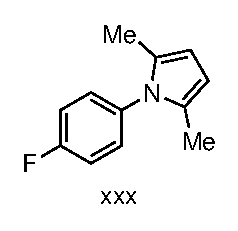
\includegraphics{exp/PMY1.eps}
	\end{center}
	\vspace{-25pt}	
	\end{figure}	

4-fluoroaniline (10.4 mL, 110 mmol, 1.1 equiv.) and 2,5-hexanedione (11.7 mL, 100 mmol, 1 equiv.) were heated to 110 $^\circ$C (oil bath temp.). After 15 hours, reaction was cooled to room temperature. The mixture was dissolved in hot EtOH (15 mL) and a mixture of EtOH (30 mL) and aqueous solution of 10\% citric acid (15 mL). The reaction was slowly cooled to approx. 10 $^\circ$C with periodic shaking. The resulting crystals were filted and washed with water (approx. 200 mL) to obtain the product as pale tan crystals (15.0 g, 79\%) after drying under vacuum at room temperature. A further crop of brown crystals (1.89 g, 10\%) could be obtained from mother liquor.
%mpt
Mpt. 48--79 (EtOH/\ce{H2O}); 
%1H
$^1$H NMR (300 MHz, \ce{CDCl3}) $\delta$ 7.21--7.11 (m, 4H), 5.89 (s, 2H), 2.01 (s, 6H); 
%13C
$^{13}$C NMR (75 MHz, \ce{CDCl3}) $\delta$ 161.9 (d, $J$ 247.4), 135.0 (d, $J$ 2.7), 129.9 (d, $J$ 8.5), 128.9, 116.0 (d, $J$ 22.6), 105.8, 12.9; 
%19F 
$^{19}$F\{$^1$H\} NMR (282 MHz, \ce{CDCl3}) $\delta$ -114.1; 
%mass spec
\emph{m/z} (APCI+) 190 [M+H]$^+$. 
%InChi
\seqsplit{InChi=1S/C12H12FN/c1-9-3-4-10(2)14(9)12-7-5-11(13)6-8-12/h3-8H,1-2H3}.
%experiment
\url{http://malaria.ourexperiment.org/uri/17}. Data consistent with literature.\url{http://dx.doi.org/10.1002/cmdc.200600026}. NMR spectra on page \pageref{spec:PMY1}.

\subsubsection*{General Prodedure B as exemplified by 1-(4-fluorophenyl)-2,5-dimethyl-1\emph{H}-pyrrole-3-carbaldehyde, OSM-S-2, PMY 2-4}
\label{exp:PMY2}
	\begin{figure}[H]
	\begin{center}
	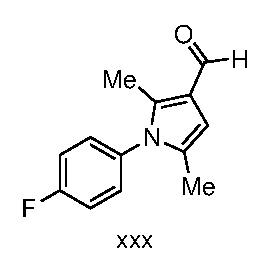
\includegraphics{exp/PMY2.eps}
	\end{center}
	\vspace{-25pt}	
	\end{figure}	

DMF (5.0 mL) was stirred under a nitrogen atmosphere in an ice-bath. Phosphoryl chloride (1.18 mL, 12.7 mmol, 1.2 equiv.) was added and the reaction stirred for 25 minutes. Reaction still colourless. A solution of pyrrole PMY 1-6 (2.00 g, 10.5 mmol, 1 equiv.) in DMF (5 mL) was added dropwise over 5 minutes. The reaction was removed from the ice-bath and allowed to warm to room temperature. After 45 minutes, reaction was complete by TLC (20\% EtOAc/hexane). The reaction was poured over ice (approx. 100 ml) and the pH adjusted to 6 (approx. 20\% /ce{NaOH(aq)}) and left stirring overnight. 20\% \ce{NaOH(aq)} added until pH 11 and left for a further 30 minutes. The solid was filtered and washed with water and recrystallised (MeCN/water) to obtain a first crop of tan free-flowing powder (2.05 g, 89\%). 
%mpt
Mpt. 117--118 $^\circ$C (MeCN/\ce{H2O}); 
%1H
$^1$H NMR (300 MHz, \ce{CDCl3}) $\delta$ 9.87 (s, 1H), 7.22--7.20 (m, 4H), 6.38 (s, 1H), 2.27 (s, 3H), 1.98 (s, 3H); 
%13C
$^{13}$C NMR (75 MHz, \ce{CDCl3}) $\delta$ 185.3, 162.5 (d, $J$ 249.7), 138.8, 132.8 (d, $J$ 2.2), 131.0, 129.7 (d, $J$ 8.7), 122.0, 116.6 (d, $J$ 22.8), 106.0, 12.6, 11.2; 
%19F
$^{19}$F\{$^1$H\} NMR (282 MHz, \ce{CDCl3}) $\delta$ xxx; 
%mass spec
\emph{m/z} (APCI+) 218 [M+H]$^+$. 
%InChi
\seqsplit{InChi=1S/C13H12FNO/c1-9-7-11(8-16)10(2)15(9)13-5-3-12(14)4-6-13/h3-8H,1-2H3}. 
%experiment
\url{ http://malaria.ourexperiment.org/uri/1f} and \url{http://www.thesynapticleap.org/node/344#comment-712}.
%data reference
Data consistent with literature.\url{http://dx.doi.org/10.1021/jm00098a013}\url{http://dx.doi.org/10.1002/cmdc.200600026} NMR spectra on page \pageref{spec:PMY2}.

\subsubsection*{Synthesis of hippuric acid, OSM-S-15, PMY 26-1}
\label{exp:PMY26}
	\begin{figure}[H]
	\begin{center}
	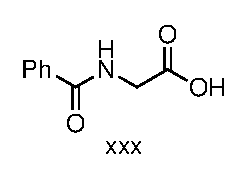
\includegraphics{exp/PMY26.eps}
	\end{center}
	\vspace{-25pt}	
	\end{figure}	

Glycine (12.5 g, 0.17 mol, 1 equiv.) was dissolved in \ce{NaOH(aq)} (13.3 g in approx 130 mL water, 0.33 mol, 2 equiv.). The flask was placed in a room temperature water bath and benzoyl chloride (21 mL, 0.18 mol, 1.06 equiv.) was added portionwise over 60 minutes keeping the temperature below 30 $^\circ$C. The reaction was stirred for an hour and then cooled in ice. Conc. \ce{HCl(aq)} (approx 20 mL) was added and the mixture stirred for 30 mins. The copious white precipitate was filtered and washed with water. The crude product was triturated with hot DCM (100 mL) for 10 minutes then filtered and washed with  further DCM (2 $\times$ 20 mL). After air drying (10 mins), the product was  dissolved in boiling water (approx 500 mL), hot filtered to remove some residual solid and allowed to crystallise slowly overnight. The crystals were filtered out (room temp.) and washed with water to obtain the product hippuric acid as white needles (22.4 g, 75\%) after drying under a stream of nitrogen.
%Mpt
Mpt. 189--190 $^\circ$C (\ce{H2O}); 
%1H
$^1$H NMR (300 MHz, \ce{CDCl3}) $\delta$ ; 
%13C
$^{13}$C NMR (75 MHz, \ce{CDCl3}) $\delta$; 
%InChi
 \seqsplit{InChi=1S/C9H9NO3/c11-8(12)6-10-9(13)7-4-2-1-3-5-7/h1-5H,6H2,(H,10,13)(H,11,12)}.
%experiment
\url{ http://malaria.ourexperiment.org/uri/5ef}.
%data reference
Data consistent with literature.\url{http://jocpr.com/vol2-iss4-2010/JCPR-2-4-410-414.pdf}\url{http://www.orgsyn.org/orgsyn/prep.asp?prep=cv2p0328}  NMR spectra on page \pageref{spec:PMY26}.

\subsubsection*{$N$-(2-((1,5-dimethyl-3-oxo-2-phenyl-2,3-dihydro-1$H$-pyrazol-4-yl)amino)-2-oxoethyl)benzamide, OSM-S-16, PMY 27-2}
\label{exp:PMY27}
	\begin{figure}[H]
	\begin{center}
	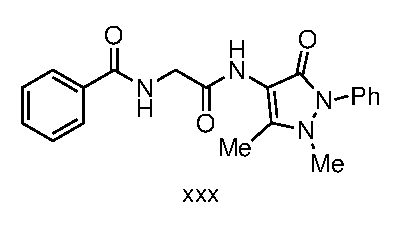
\includegraphics{exp/PMY27.eps}
	\end{center}
	\vspace{-25pt}	
	\end{figure}	

Prepared according to literature method.\url{http://www.ncbi.nlm.nih.gov/pubmed/8267666}

%Mpt
Mtp. xxx $^\circ$C;
%1H
$^1$H NMR (300 MHz, \ce{CDCl3}) $\delta$ ; 
%13C
$^{13}$C NMR (75 MHz, \ce{CDCl3}) $\delta$;
%IR
 $\nu_{max}$ (neat) /$cm^{-1}$ ;
%mass spec
\emph{m/z} (ESI+) [M+H]$^+$.
%InChi
\seqsplit{InChi=1S/C20H20N4O3/c1-14-18(20(27)24(23(14)2)16-11-7-4-8-12-16)22-17(25)13-21-19(26)15-9-5-3-6-10-15/h3-12H,13H2,1-2H3,(H,21,26)(H,22,25)}.
%experiment
\url{http://malaria.ourexperiment.org/uri/75}.
%data reference
 See page \pageref{spec:PMY27} for NMR spectra. Data consistent with literature.\url{http://www.ncbi.nlm.nih.gov/pubmed/8267666}

\subsubsection*{OSM-S-17, PMY 29-1, PMY 29-2}
\label{exp:PMY29}
	\begin{figure}[H]
	\begin{center}
	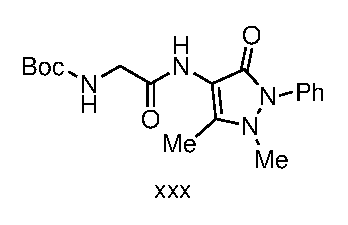
\includegraphics{exp/PMY29.eps}
	\end{center}
	\vspace{-25pt}	
	\end{figure}	

%Mpt
Mtp. xxx $^\circ$C;
%1H
$^1$H NMR (300 MHz, \ce{CDCl3}) $\delta$ ; 
%13C
$^{13}$C NMR (75 MHz, \ce{CDCl3}) $\delta$;
%IR
 $\nu_{max}$ (neat) /$cm^{-1}$ ;
%mass spec
\emph{m/z} (ESI+) [M+H]$^+$.
%InChi
\seqsplit{InChi=1S/C18H24N4O4/c1-12-15(20-14(23)11-19-17(25)26-18(2,3)4)16(24)22(21(12)5)13-9-7-6-8-10-13/h6-10H,11H2,1-5H3,(H,19,25)(H,20,23)}.
%experiment
\url{http://malaria.ourexperiment.org/uri/6c}.
%data reference
 See page \pageref{spec:PMY29} for NMR spectra. Data consistent with literature.\url{http://dx.doi.org/10.1007/s00726-008-0074-1}

\subsubsection*{$N$-(1,5-Dimethyl-3-oxo-2-phenyl-2,3-dihydro-1$H$-pyrazol-4-yl)glycinamide, OSM-S-18, PMY 30-3}
\label{exp:PMY30}
	\begin{figure}[H]
	\begin{center}
	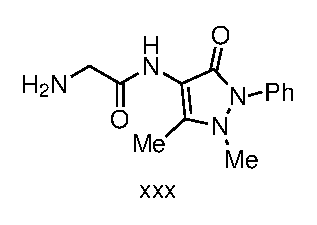
\includegraphics{exp/PMY30.eps}
	\end{center}
	\vspace{-25pt}	
	\end{figure}	

%Mpt
Mtp. xxx $^\circ$C;
%1H
$^1$H NMR (300 MHz, \ce{CDCl3}) $\delta$ ; 
%13C
$^{13}$C NMR (75 MHz, \ce{CDCl3}) $\delta$;
%IR
 $\nu_{max}$ (neat) /$cm^{-1}$ ;
%mass spec
\emph{m/z} (ESI+) [M+H]$^+$.
%InChi
\seqsplit{InChi=1S/C13H16N4O2/c1-9-12(15-11(18)8-14)13(19)17(16(9)2)10-6-4-3-5-7-10/h3-7H,8,14H2,1-2H3,(H,15,18)}.
%experiment
\url{http://malaria.ourexperiment.org/uri/8d}.
%data reference
 See page \pageref{spec:PMY30} for NMR spectra. Data consistent with literature.\url{http://www.ncbi.nlm.nih.gov/pubmed/8267666}


%\subsubsection*{OSM-S-23, PMY 43-1}

%\subsubsection*{OSM-S-24, PMY 44-1}

\subsubsection*{OSM-S-25, LMW 1}
\label{exp:LMW1}
	\begin{figure}[H]
	\begin{center}
	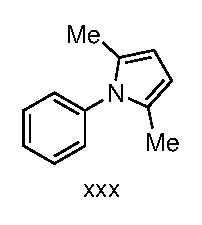
\includegraphics{exp/LMW1.eps}
	\end{center}
	\vspace{-25pt}	
	\end{figure}	

%Mpt
Mtp. 49--50 $^\circ$C;
%1H
$^1$H NMR (300 MHz, \ce{CDCl3}) $\delta$ 7.44--7.36 (s, 3H), 7.21--7.17 (t, 2H), 5.90 (s, 2H), 2.02 (s, 6H); 
%13C
$^{13}$C NMR (75 MHz, \ce{CDCl3}) $\delta$ 139.1, 129.1. 128.8, 128.3, 127.7, 105.8, 13.1;
%IR
 $\nu_{max}$ (neat) /$cm^{-1}$ 1597, 1520, 1494, 1401, 1318, 1037, 1006, 773, 747, 717, 695, 646;
%mass spec
\emph{m/z} (APCI) 173 [M+H]$^+$.
%InChi
\seqsplit{InChi=1S/C12H13N/c1-10-8-9-11(2)13(10)12-6-4-3-5-7-12/h3-9H,1-2H3}.
%experiment
\url{http://malaria.ourexperiment.org/uri/4c}.
%data reference
 See page \pageref{spec:LMW1} for NMR spectra. Data consistent with literature.\url{http://dx.doi.org/10.1002/cmdc.200600026}

\subsubsection*{OSM-S-26, LMW 2}
\label{exp:LMW2}
	\begin{figure}[H]
	\begin{center}
	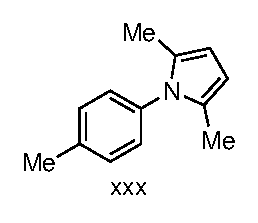
\includegraphics{exp/LMW2.eps}
	\end{center}
	\vspace{-25pt}	
	\end{figure}	

%Mpt
Mtp. 45--46 $^\circ$C;
%1H
$^1$H NMR (300 MHz, \ce{CDCl3}) $\delta$ 7.23--7.20 (m, 2H), 7.08--7.05 (m, 2H), 5.88 (s, 2H), 2.38 (s, 3H), 2.01 (s, 6H);
%13C
$^{13}$C NMR (75 MHz, \ce{CDCl3}) $\delta$ 137.5, 136.6, 129.8, 128.9, 128.1, 105.7, 21.3, 13.2;
%IR
 $\nu_{max}$ (neat) /$cm^{-1}$ 1513.22, 1403, 1320, 826, 750;
%mass spec
\emph{m/z} (ESI+) 187 [M+H]$^+$.
%InChi
\seqsplit{InChi=1S/C13H15N/c1-10-4-8-13(9-5-10)14-11(2)6-7-12(14)3/h4-9H,1-3H3}.
%experiment
\url{http://malaria.ourexperiment.org/uri/4b}.
%data reference
 See page \pageref{spec:LMW2} for NMR spectra. Data consistent with literature.\url{http://dx.doi.org/10.1002/cmdc.200600026}


\subsubsection*{OSM-S-27, LMW 3}
\label{exp:LMW3}
	\begin{figure}[H]
	\begin{center}
	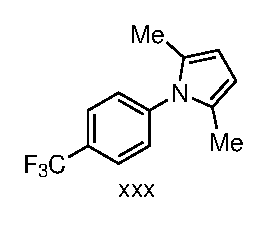
\includegraphics{exp/LMW3.eps}
	\end{center}
	\vspace{-25pt}	
	\end{figure}	

%Mpt
Mtp. 70--73 $^\circ$C;
%1H
$^1$H NMR (300 MHz, \ce{CDCl3}) $\delta$ 7.73 (d, $J$ 8.2, 2H), 7.34 (d, $J$ 8.3), 5.93 (s, 2H), 2.05 (s, 6H); 
%13C
$^{13}$C NMR (75 MHz, \ce{CDCl3}) $\delta$  142.3, 129.8 (q, $J$ 32.7), 128.1, 128.6, 126.3 (m), 123.9 (q, $J$ 272.1), 106.6, 13.0;
%IR
 $\nu_{max}$ (neat) /$cm^{-1}$ 1615, 1402, 1325, 1128, 1064, 850, 759;
%mass spec
\emph{m/z} (ESI+) 241 [M+H]$^+$.
%InChi
\seqsplit{InChi=1S/C13H12F3N/c1-9-3-4-10(2)17(9)12-7-5-11(6-8-12)13(14,15)16/h3-8H,1-2H3}.
%experiment
\url{http://malaria.ourexperiment.org/uri/4a}.
%data reference
 See page \pageref{spec:LMW2} for NMR spectra. Data consistent with literature.\url{http://dx.doi.org/10.1002/cmdc.200600026}


\subsubsection*{2,5-dimethyl-1$H$-phenyl pyrrole-3-carboxaldehyde, OSM-S-28, LMW 4}
\label{exp:LMW4}
	\begin{figure}[H]
	\begin{center}
	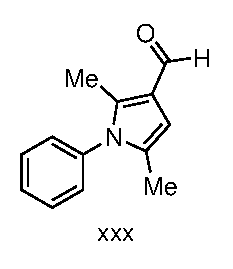
\includegraphics{exp/LMW4.eps}
	\end{center}
	\vspace{-25pt}	
	\end{figure}	

=== standardise ===

Prepared according to General Procedure B using DMF (1.5 mL, 19.4 mmol, 6.5 equiv.) was stirred under a nitrogen atmosphere in an ice-bath. Phosphoryl chloride (0.308 mL, 3.3 mmol, 1.1 equiv.) was added and the reaction stirred for 30 minutes. Reaction mixture was a very pale yellow. A solution of 2,5-dimethyl-1H-phenyl-pyrrole (514 mg, 3 mmols, 1 equiv.) in DMF (2 mL) was added dropwise over 1 minute. After 5 minutes, the flask was removed from ice and reaction stirred for a further 55 mins. TLC at 1 hr showed reaction to be complete. Reaction mixture was poured onto ice (50 mL) and 1M NaOH added (pH 11), until adjusted to pH 6. Total volume approximately 50 mL after ice has melted and was pH 3 the next day. 20\% NaOH was added to achieve pH 11 and flask bathed in a brine ice-bath for 20 minutes. Product was filtered and washed with water to produce a wet brown paste. Product was dissolved in MeCN and concentrated under a nitrogen atmosphere. Brown-green solution with slight precipitation was observed overnight. Product was then extracted using a mixture of EtOAc (2 × 20 mL), Et2O (20 mL), water (20 mL) and brine (20 mL). Product was concentrated under reduced pressure and cooled in refrigerator overnight to crystallise. Product was dissolved in EtOH (3 mL) in a water bath at 40°C. Solution was cooled in a brine ice bath and filtered. Filter cake was washed with water (3 × 10 mL) and product dried under vacuum to give a grey free-flowing powder (407 mg, 64\%).
%Mpt
Mtp. 88--90 $^\circ$C;
%1H
$^1$H NMR (300 MHz, \ce{CDCl3}) $\delta$  9.88 (s, 1H), 7.55--7.50 (m, 3H), 7.22--7.19 (m, 2H), 6.39 (s, 1H), 2.28 (s, 3H), 1.99 (s, 3H); 
%13C
$^{13}$C NMR (75 MHz, \ce{CDCl3}) $\delta$ 185.3, 138.9, 137.0, 131.0, 129.6, 128.9, 128.0, 121.9, 105.8, 12.7, 11.2;
%IR
 $\nu_{max}$ (neat) /$cm^{-1}$ 1650, 1422, 801, 669;
%mass spec
\emph{m/z} (ESI+) 200 [M+H]$^+$.
%InChi
\seqsplit{InChi=1S/C13H13NO/c1-10-8-12(9-15)11(2)14(10)13-6-4-3-5-7-13/h3-9H,1-2H3}.
%experiment
\url{http://malaria.ourexperiment.org/uri/4d}.
%data reference
 See page \pageref{spec:LMW4} for NMR spectra. Data consistent with literature.\url{http://dx.doi.org/10.1002/cmdc.200600026}

\subsubsection*{2,5-dimethyl-1$H$-($p$-tolyl)-pyrrole-3-carboxaldehyde, OSM-S-29, LMW 5}
\label{exp:LMW5}
	\begin{figure}[H]
	\begin{center}
	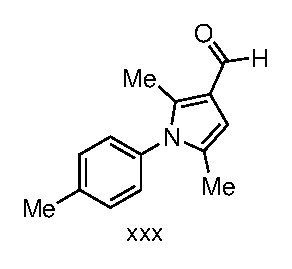
\includegraphics{exp/LMW5.eps}
	\end{center}
	\vspace{-25pt}	
	\end{figure}	

=== standardise ===

Prepared according to General Procedure B
 DMF (1.5 mL, 19.4 mmol, 6.5 equiv.) was stirred under a nitrogen atmosphere in an ice-bath. Phosphoryl chloride (0.308 mL, 3.3 mmol, 1.1 equiv.) was added and the reaction stirred for 30 minutes. Reaction mixture was a very pale yellow. A solution of 2,5-dimethyl-1H-(p-tolyl)-pyrrole (556 mg, 3 mmols, 1 equiv.) in DMF (2 mL) was added dropwise over 1 minute. After 5 minutes, flask removed from ice and reaction stirred for a further 55 mins. TLC at 1 hr showed reaction at completion. Reaction mixture was then poured onto ice (50 mL) and 1M NaOH added (pH 11), until adjusted to pH 6. Total volume approximately 50 mL after ice has melted and solution was pH 3 the next day. 20\% NaOH was added to achieve pH 11 and flask bathed in a brine ice-bath for 20 minutes. Product filtered and washed with water to produce a wet brown paste. Product was dissolved in MeCN and concentrated under a nitrogen atmosphere. Brown solution with precipitation of fine crystals was observed overnight. Solution was cooled in an ice bath and filtered. Filter cake washed with water (3 $\times$ 10 mL). Filtered product was then dried under vacuum to produce a lumpy grey-brown powder (423 mg, 71\%).
%Mpt
Mtp. 109--111 $^\circ$C;
%1H
$^1$H NMR (300 MHz, \ce{CDCl3}) $\delta$  9.86 (s, 1H), 7.31 (d, $J$ 7.9, 2H), 7.07 (d, $J$ 7.9, 2H), 6.37 (s, 1H), 2.44 (s, 3H), 2.27 (s, 3H), 1.98 (s, 3H); 
%13C
$^{13}$C NMR (75 MHz, \ce{CDCl3}) $\delta$185.2, 139.0, 138.9, 134.3, 131.1, 130.2, 127.7, 121.8, 105.6, 21.2, 12.6, 11.2; 
%IR
 $\nu_{max}$ (neat) /$cm^{-1}$  3935, 1651, 1515, 1422, 811;
%mass spec
\emph{m/z} (ESI+) 214 [M+H]$^+$.
%InChi
\seqsplit{InChi=1S/C14H15NO/c1-10-4-6-14(7-5-10)15-11(2)8-13(9-16)12(15)3/h4-9H,1-3H3}.
%experiment
\url{http://malaria.ourexperiment.org/uri/4e}.
%data reference
See page \pageref{spec:LMW5} for NMR spectra.
 Data consistent with literature.\url{http://dx.doi.org/10.1002/cmdc.2006000265}

\subsubsection*{ Synthesis of ethyl 2,5-dimethyl-1-phenyl-1$H$-pyrrole-3-carboxylate, OSM-S-31, LMW 8-1}
	\label{exp:LMW8}
	\begin{figure}[H]
	\begin{center}
	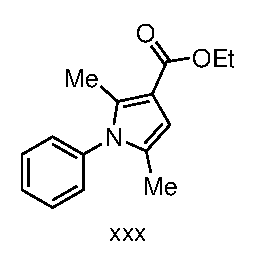
\includegraphics{exp/LMW8.eps}
	\end{center}
	\vspace{-25pt}	
	\end{figure}	

=== standardise ===

Prepared according to general method C using ethyl acetoacetate (6 mL,47 mmol, 1 equiv.) and \ce{K2CO3} (8.45 g, 61.1 mmol, 1.3 equiv.) were mixed in MeCN (55 mL). NaI (7.05 g, 47 mmol, 1 equiv.) and chloroacetone (4.8 mL, 51.7 mmol, 1.1 equiv.) were added and mixture heated to 80 $^\circ$C in an oil bath. TLC at 2 hours showed reaction at completion. Reaction was allowed to cool to room temperature. Mixture washed with EtOAc (2 $\times$ 20 mL), water (2 $\times$ 20 mL), 1:1 water:brine (2 $\times$ 20 mL) and brine (2 $\times$ 20 mL) and dried with MgSO4 and concentrated under reduced pressure to form a yellow oil. Ethyl 2-acetyl-4-oxopentanoate intermediate (2 mL, 10.7 mmol, 1 equiv.) was added to aniline (1.17 mL, 12.89 mmol, 1.2 equiv.) and heated at 80 $^\circ$C in an oil bath for 75 mins. TLC at 1 hour showed reaction at completion and reaction was allowed to cool to room temperature. Product was washed with EtOAc (2 $\times$ 20 mL), 10\% citric acid (3 $\times$ 20 mL), water (20 mL) and brine (2 $\times$ 20 mL) and then concentrated under reduced pressure to form a dark brown oil. Product was purified by chromatography on silica (2-15\% EtOAc/petrol). Product containing fractions concentrated under reduce pressure to produce a yellow oil (952 mg, approximate yield 37\%) which was used without further purification.

%1H
$^1$H NMR (300 MHz, \ce{CDCl3}) $\delta$  7.50--7.41 (m, 2H), 7.18--7.15 (m, 2H), 6.38 (s, 1H), 4.28 (q, $J$ 7.1, 2H), 2.29 (s, 3H), 1.97 (s, 3H), 1.34 (t, $J$ 7.1, 3H); 
%13C
$^{13}$C NMR (75 MHz, \ce{CDCl3}) $\delta$ 165.7, 137.8, 136.2, 129.4, 128.7, 128.5, 128.2, 111.5, 107.6, 59.2, 14.6, 12.6, 12.4; 
%IR
 $\nu_{max}$ (neat) /$cm^{-1}$ 2978, 1693, 1411, 121;
%mass spec
\emph{m/z} (APCI+) 244 [M+H]$^+$.
%InChi
\seqsplit{InChi=1S/C15H17NO2/c1-4-18-15(17)14-10-11(2)16(12(14)3)13-8-6-5-7-9-13/h5-10H,4H2,1-3H3}.
%experiment
\url{http://malaria.ourexperiment.org/uri/50}.
%data reference
Data consistent with literature.\url{http://dx.doi.org/10.1016/0040-4020(80)80102-5}

\subsubsection*{OSM-S-41, ZYH 9-1}
\label{exp:ZYH9}
	\begin{figure}[H]
	\begin{center}
	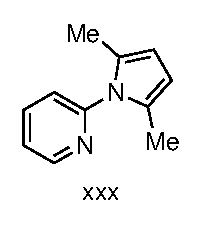
\includegraphics{exp/ZYH9.eps}
	\end{center}
	\vspace{-25pt}	
	\end{figure}	

Prepared according to General Procedure A except

%1H
$^1$H NMR (300 MHz, \ce{CDCl3}) $\delta$ ; 
%13C
$^{13}$C NMR (75 MHz, \ce{CDCl3}) $\delta$;
%IR
 $\nu_{max}$ (neat) /$cm^{-1}$ ;
%mass spec
\emph{m/z} (ESI+) [M+H]$^+$.
%InChi
\seqsplit{InChi=1S/C11H12N2/c1-9-6-7-10(2)13(9)11-5-3-4-8-12-11/h3-8H,1-2H3}.
%experiment
\url{http://malaria.ourexperiment.org/uri/60}.
%data reference
 See page \pageref{spec:ZYH9} for NMR spectra. Data consistent with literature.\url{http://dx.doi.org/10.1590/S0103-50532008000500011}

\subsubsection*{OSM-S-53, ZYH 20-1}
\label{exp:ZYH20}
	\begin{figure}[H]
	\begin{center}
	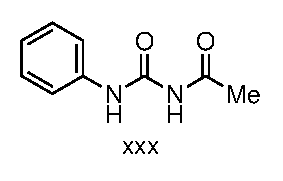
\includegraphics{exp/ZYH20.eps}
	\end{center}
	\vspace{-25pt}	
	\end{figure}

%Mpt
Mtp. 166--167 $^\circ$C;
%1H
$^1$H NMR (300 MHz, \ce{CDCl3}) $\delta$ ; 
%13C
$^{13}$C NMR (75 MHz, \ce{CDCl3}) $\delta$;
%IR
 $\nu_{max}$ (neat) /$cm^{-1}$ ;
%mass spec
\emph{m/z} (ESI+) [M+H]$^+$.
%InChi
\seqsplit{InChi=1S/C9H10N2OS/c1-7(12)10-9(13)11-8-5-3-2-4-6-8/h2-6H,1H3,(H2,10,11,12,13)}.
%experiment
\url{http://malaria.ourexperiment.org/uri/7b}.
%data reference
See page \pageref{spec:ZYH20} for NMR spectra. Data consistent with literature.\url{http://dx.doi.org/10.1080/03086647708079937}

\subsubsection*{OSM-S-55, ZYH 23-1}
\label{exp:ZYH23}
	\begin{figure}[H]
	\begin{center}
	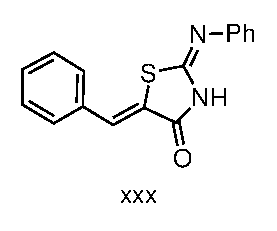
\includegraphics{exp/ZYH23.eps}
	\end{center}
	\vspace{-25pt}	
	\end{figure}

Prepared according to literature.\url{http://dx.doi.org/10.1016/j.bmc.2008.10.032}

%Mpt
Mtp. 260--261 $^\circ$C;
%1H
$^1$H NMR (300 MHz, \ce{CDCl3}) $\delta$ ; 
%13C
$^{13}$C NMR (75 MHz, \ce{CDCl3}) $\delta$;
%IR
 $\nu_{max}$ (neat) /$cm^{-1}$ ;
%mass spec
\emph{m/z} (ESI+) 303 [M+Na]$^+$.
%InChi
\seqsplit{InChi=1S/C16H12N2OS/c19-15-14(11-12-7-3-1-4-8-12)20-16(18-15)17-13-9-5-2-6-10-13/h1-11H,(H,17,18,19)/b14-11-}.
%experiment
\url{http://malaria.ourexperiment.org/uri/85}.
%data reference
See page \pageref{spec:ZYH23} for NMR spectra. Data consistent with literature.\url{http://dx.doi.org/10.1016/j.bmc.2008.10.032}

\section{Novel compounds or those without reported\\ experimental data}

\subsubsection*{General procedure C for the synthesis of pyrrole-3-esters as exemplified by ethyl 1-(4-fluorophenyl)-2,5-dimethyl-1$H$-pyrrole-3-carboxylate, OSM-S-3, PMY 6-1}
\label{exp:PMY6}
	\begin{figure}[H]
	\begin{center}
	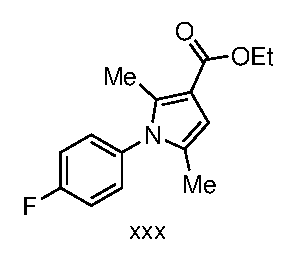
\includegraphics{exp/PMY6.eps}
	\end{center}
	\vspace{-25pt}	
	\end{figure}	

Ethyl acetoacetate (2.00 mL, 15.7 mmol, 1 equiv.) and \ce{K2CO3} (2.82 g, 20.4 mmol, 1.3 equiv.) in acetonitrile (30 mL) were cooled ice/brine. Chloroacetone (1.39, 17.2 mmol, 1.1 equiv.) was added dropwise. After stirring for 15 minutes, reaction was allowed to warm to room temperature. After 15 minutes, sodium iodide (2.58 g, 17.2 mmol, 1.1 equiv.) was added. After stirring for a further for 1.5 hours, reaction is now a pale yellow suspension  Heated to reflux. After 20 hours at reflux, reaction was allowed to cool and then filtered. The filtrate was concentrated under reduced pressure and then dissolved in EtOAc (40 mL). Washed with water (2 $\times$ 20 mL), 1:1 brine/water (20 mL) to break emulsion, brine and dried (\ce{MgSO4}) then concentrated under reduced pressure to a brown oil (2.95 g). $^1$H NMR consistent with product\url{http://dx.doi.org/10.1021/jo00391a003} which was used without further purification. 

4-fluoroaniline (1.78 mL, 18.8 mmol, 1.2 equiv.) was added and the reaction heated to 90 $^\circ$C. After 2 hours, reaction complete by TLC. Reaction cooled. Black oil with colouless liquid (water). Dissolved in EtOAc (30 mL) and washed with 10\% citric acid (3 $\times$ 15 mL), water (3 $\times$ 15 mL) and brine then dried (\ce{MgSO4}) and concentrated under reduced pressure (3.70 g). Recrystallised EtOH/water; Dissolved in warm EtOH (4 mL) and cooled in ice until crystallisation initiated, then 40\% EtOH (16 mL) added slowly with stirring. Cooled in ice for 30 minutes to complete crystallisation and filtered. Red/brown crystals washed with 20\% EtOH and dried under vacuum (2.77 g, 61\% over 2 steps). 
%Mpt
Mpt. 63--66 $^\circ$C (\ce{EtOH}/\ce{H2O}); 
%1H
$^1$H NMR (300 MHz, \ce{CDCl3}) $\delta$ 7.19--7.16 (m, 4H), 6.37 (s, 1H), 4.28 (q, $J$ 7.1, 2H), 2.28 (s, 3H), 1.96 (s, 3H), 1.34 (d, $J$ 7.1, 3H); 
%13C
  $^{13}$C NMR (75 MHz, \ce{CDCl3}) $\delta$ 165.6, 162.3 (d, $J$ 248.8), 136.2, 133.7 (d, $J$2.9), 129.9 (d, $J$ 8.7), 128.8, 116.4 (d, $J$ 22.8), 111.6, 107.6, 59.3, 14.5, 12.6, 12.3; 
 %IR
 $\nu_{max}$ (neat) /$cm^{-1}$ ; 
%mass
\emph{m/z} (ESI+) xxx [M+H]$^+$.
%InChi
\seqsplit{InChi=1S/C15H16FNO2/c1-4-19-15(18)14-9-10(2)17(11(14)3)13-7-5-12(16)6-8-13/h5-9H,4H2,1-3H3}.
%experiment
 See page \pageref{spec:PMY6} for NMR spectra. \url{ http://malaria.ourexperiment.org/uri/20}. 

\subsubsection*{ General Procedure D for hydrolysis of pyrrole-3-esters to their corresponding acids as exemplified by 1-(4-fluorophenyl)-2,5-dimethyl-1$H$-pyrrole-3-carboxylic acid, OSM-S-4, PMY 8}
\label{exp:PMY8}
	\begin{figure}[H]
	\begin{center}
	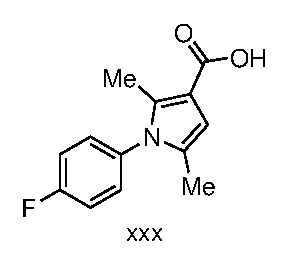
\includegraphics{exp/PMY8.eps}
	\end{center}
	\vspace{-25pt}	
	\end{figure}	

PMY 6 (2.16 g, 8.27 mmol, 1 equiv.) was dissolved in EtOH (approx 30 mL) and 20\% \ce{NaOH(aq)} (40 mL, approx 17 equiv.). The reaction was heated to reflux for approximately 16 hours. The reaction was then cooled in ice and  15\% \ce{HCl} was added slowly until a pale precipitate formed (pH 1). The mixture was stirred for a further 15 minutes and then filtered. The pale brown cake was washed with water (2 $\times$ 25 mL). After drying under vacuum the product was obtained as a pale brown powder (1.73 g, 89\%).
%Mpt
Mpt.241--242$^\circ$C (acetone/\ce{H2O}) decomposition; 
%1H
$^1$H NMR (300 MHz, \ce{CDCl3}) $\delta$ 7.19 (app d, $J$ 6.4, 4H), 6.42 (br s, 1H), 2.30 (s, 3H), 1.97 (s, 3H); 
%13C
  $^{13}$C NMR (75 MHz, \ce{CDCl3}) $\delta$ 171.09, 162.4 (d, $J$ 249.0), 137.8, 133.6 (d, $J$ 2.7), 129.9 (d, $J$ 8.6), 129.2, 116.5 (d, $J$ 22.8), 110.8, 108.2, 12.6, 12.5; 
 %IR
 $\nu_{max}$ (neat) /$cm^{-1}$ ; 
%mass
\emph{m/z} (ESI+) xxx [M+H]$^+$.
%InChi
\seqsplit{InChi=1S/C13H12FNO2/c1-8-7-12(13(16)17)9(2)15(8)11-5-3-10(14)4-6-11/h3-7H,1-2H3,(H,16,17)}. 
%experiment
 See page \pageref{spec:PMY8} for NMR spectra. \url{http://malaria.ourexperiment.org/uri/81}. 

\subsubsection*{General Procedure E for the Synthesis of pyrrole 3-esters or amides as exemplified by 2-amino-2-oxoethyl 1-(4-fluorophenyl)-2,5-dimethyl-1$H$-pyrrole-3-carboxylate, TCMDC-123812, OSM-S-5, PMY 10}
\label{exp:PMY10}
	\begin{figure}[H]
	\begin{center}
	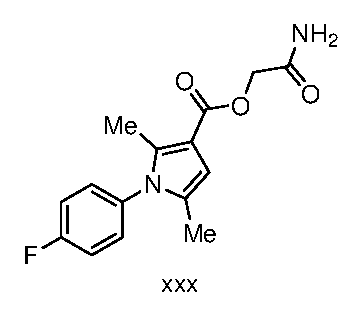
\includegraphics{exp/PMY10.eps}
	\end{center}
	\vspace{-25pt}	
	\end{figure}	

%Mpt
Mpt.xxx--xxx $^\circ$C (xxx); 
%1H
$^1$H NMR (300 MHz, \ce{CDCl3}) $\delta$ 7.21--7.17 (m, 4H), 6.37 (s, 1H), 6.03 (app br d, $J$ 70.2, 2H), 4.74 (s, 2H), 2.30 (s, 3H), 1.98 (s, 3H); 
%13C
  $^{13}$C NMR (75 MHz, \ce{CDCl3}) $\delta$ 171.1, 163.7, 162.5 (d, $J$ 249.3), 137.8, 133.3 (d, $J$ 3.4), 129.8 (d, $J$ 8.7), 129.4, 116.6 (d, $J$ 23.0), 109.9, 107.4, 61.8, 12.6, 12.4; 
%19F
$^{19}$F\{$^1$H\} NMR (282 MHz, \ce{CDCl3}) $\delta$ -111.92;
 %IR
 $\nu_{max}$ (neat) /$cm^{-1}$ ; 
%mass
\emph{m/z} (ESI+) xxx [M+H]$^+$.
%InChi
\seqsplit{InChi=1S/C15H15FN2O3/c1-9-7-13(15(20)21-8-14(17)19)10(2)18(9)12-5-3-11(16)4-6-12/h3-7H,8H2,1-2H3,(H2,17,19)}. 
%experiment
See page \pageref{spec:PMY10} for NMR spectra.
\url{http://malaria.ourexperiment.org/xxx}. 


\subsubsection*{TCMDC-123794, OSM-S-6, PMY 11-2}
\label{exp:PMY11}
	\begin{figure}[H]
	\begin{center}
	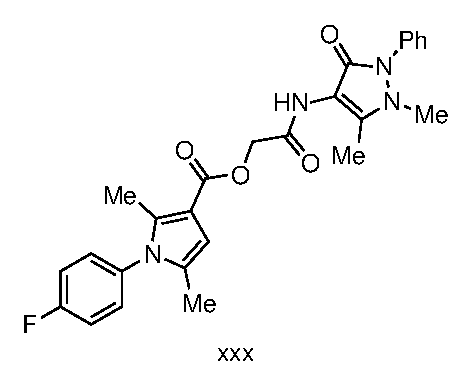
\includegraphics{exp/PMY11.eps}
	\end{center}
	\vspace{-25pt}	
	\end{figure}	
General procedure E

%Mpt
Mpt.xxx--xxx $^\circ$C (xxx); 
%1H
$^1$H NMR (300 MHz, \ce{CDCl3}) $\delta$ 7.64 (br s, 1H), 7.48--7.37 (m, 4H), 7.32--7.30 (m, 1H), 7.21--7.16 (m, 4H), 6.43 (s, 1H), 4.87 (s, 2H), 3.08 (s, 3H), 2.31 (s, 6H), 1.95 (s, 3H); 
%13C
  $^{13}$C NMR (75 MHz, \ce{CDCl3}) $\delta$ ok but need a stronger one; 
%19F
$^{19}$F\{$^1$H\} NMR (282 MHz, \ce{CDCl3}) $\delta$ -112.14; 
%IR
 $\nu_{max}$ (neat) /$cm^{-1}$ ; 
%mass
\emph{m/z} (ESI+) xxx [M+H]$^+$.
%InChi
\seqsplit{InChi=1S/C26H25FN4O4/c1-16-14-22(17(2)30(16)20-12-10-19(27)11-13-20)26(34)35-15-23(32)28-24-18(3)29(4)31(25(24)33)21-8-6-5-7-9-21/h5-14H,15H2,1-4H3,(H,28,32)}. 
%experiment
\url{http://malaria.ourexperiment.org/xxx}. 

\subsubsection*{OSM-S-7, PMY 12-1}
\label{exp:PMY12-1}
	\begin{figure}[H]
	\begin{center}
	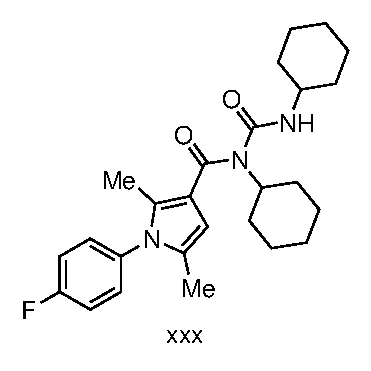
\includegraphics{exp/PMY12-1.eps}
	\end{center}
	\vspace{-25pt}	
	\end{figure}	

DCC coupling

%Mpt
Mpt.xxx--xxx $^\circ$C (xxx); 
%1H
$^1$H NMR (300 MHz, \ce{CDCl3}) $\delta$ 7.22--7.11 (m, 4H), 6.54 (br app d, $J$ 7.3, rotamers, 1H), 6.10 (s, 1H), 4.26 (br t, $J$ 11.8, 1H), 3.69--3.61 (m, 1H), 2.22--2.11 (m, 5H), 1.95 (br s, 3H), 1.83--1.79 (m, 6H), 1.63-1.55 (m, 4H), 1.37--1.08 (m, 8H); 
%13C
  $^{13}$C NMR (75 MHz, \ce{CDCl3}) $\delta$ 169.5, 162.3 (d, $J$ 248.9), 15534, 134.0, 133.7 (d, $J$ 2.2), 129.8 (d, $J$ 8.7), 128.7, 116.4 (d, $J$ 23.2), 116.3, 106.1, 57.7, 49.3, 32.6, 31.1, 26.4, 25.6, 25.4, 24.5, 12.5, 12.2; 
%19F
$^{19}$F\{$^1$H\} NMR (282 MHz, \ce{CDCl3}) $\delta$ -112.41; 
 %IR
 $\nu_{max}$ (neat) /$cm^{-1}$ ; 
%mass
\emph{m/z} (ESI+) xxx [M+H]$^+$.
%InChi
\seqsplit{InChi=1S/C26H34FN3O2/c1-18-17-24(19(2)29(18)23-15-13-20(27)14-16-23)25(31)30(22-11-7-4-8-12-22)26(32)28-21-9-5-3-6-10-21/h13-17,21-22H,3-12H2,1-2H3,(H,28,32)}. 
%experiment
See page \pageref{spec:PMY12-1} for NMR spectra.\url{http://malaria.ourexperiment.org/uri/30}. 

\subsubsection*{OSM-S-8, PMY 12-5}
 \label{exp:PMY12-5}
	\begin{figure}[H]
	\begin{center}
	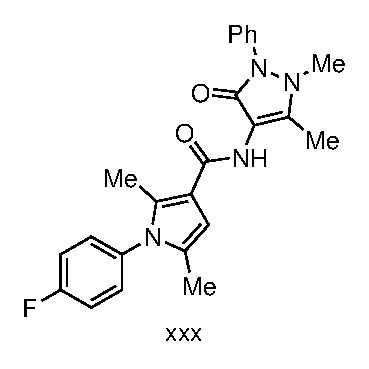
\includegraphics{exp/PMY12-5.eps}
	\end{center}
	\vspace{-25pt}	
	\end{figure}	

T3P coupling

%Mpt
Mpt.xxx--xxx $^\circ$C (xxx); 
%1H
$^1$H NMR (300 MHz, \ce{CDCl3}) $\delta$ 4.50--7.39 (m, 4H), 7.33--7.29 (m, 1H), 7.19--7.15 (m, 4H), 6.28 (s, 1H), 2.86 (s, 3H), 2.33 (s, 3H), 2.30 (s, 3H), 1.97 (s, 3H); 
%13C
  $^{13}$C NMR (75 MHz, \ce{CDCl3}) $\delta$ ; 
%19F
$^{19}$F\{$^1$H\} NMR (282 MHz, \ce{CDCl3}) $\delta$ xxx; 
 %IR
 $\nu_{max}$ (neat) /$cm^{-1}$ ; 
%mass
\emph{m/z} (ESI+) xxx [M+H]$^+$.
%InChi
\seqsplit{InChi=1S/C24H23FN4O2/c1-15-14-21(16(2)28(15)19-12-10-18(25)11-13-19)23(30)26-22-17(3)27(4)29(24(22)31)20-8-6-5-7-9-20/h5-14H,1-4H3,(H,26,30)}. 
%experiment
\url{http://malaria.ourexperiment.org/uri/65}. 

\subsubsection*{OSM-S-9, PMY 14-4}
\label{exp:PMY14}
	\begin{figure}[H]
	\begin{center}
	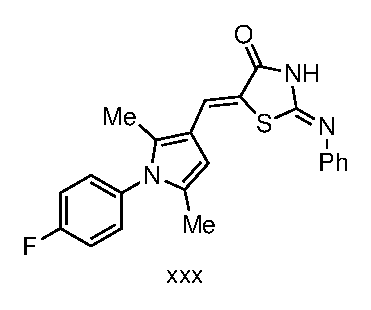
\includegraphics{exp/PMY14.eps}
	\end{center}
	\vspace{-25pt}	
	\end{figure}	

Prepared according to literature procedure.\url{http://dx.doi.org/10.1016/j.bmcl.2011.09.049}

%Mpt
Mpt.xxx--xxx $^\circ$C (xxx); 
%1H
$^1$H NMR (300 MHz, \ce{CDCl3}) $\delta$ ; 
%13C
  $^{13}$C NMR (75 MHz, \ce{CDCl3}) $\delta$ ; 
%19F
$^{19}$F\{$^1$H\} NMR (282 MHz, \ce{CDCl3}) $\delta$ xxx; 
 %IR
 $\nu_{max}$ (neat) /$cm^{-1}$ ; 
%mass
\emph{m/z} (ESI+) 434 [M+Na]$^+$.
%InChi
\seqsplit{InChI=1S/C22H18FN3OS/c1-14-12-16(15(2)26(14)19-10-8-17(23)9-11-19)13-20-21(27)25-22(28-20)24-18-6-4-3-5-7-18/h3-13H,1-2H3,(H,24,25,27)/b20-13-}. 
%experiment
\url{http://malaria.ourexperiment.org/uri/33}. 

\subsubsection*{General Procedure F as exemplified by (2$Z$,5$Z$)-5-((1-(4-fluorophenyl)-2,5-dimethyl-1$H$-pyrrol-3-yl)methylene)-2-(phenylimino)thiazolidin-4-one, OSM-S-10, PMY 35}
 \label{exp:PMY35}
	\begin{figure}[H]
	\begin{center}
	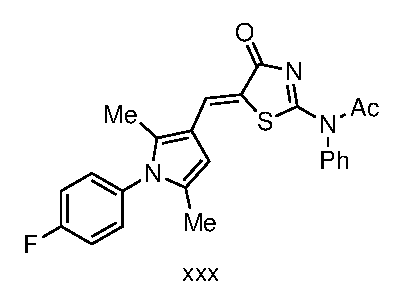
\includegraphics{exp/PMY35.eps}
	\end{center}
	\vspace{-25pt}	
	\end{figure}	

Prepared according to method reported by Roberts.\url{http://dx.doi.org/10.1016/j.bmc.2008.10.032}


%Mpt
Mpt.xxx--xxx $^\circ$C (xxx); 
%1H
$^1$H NMR (300 MHz, \ce{CDCl3}) $\delta$ 7.95 (s, 1H), 7.53--7.50 (m, 3H), 7.32--7.18 (m, 6H), 6.40 (s, 1H), 2.16 (s, 3H), 2.12 (s, 3H), 2.04 (s, 3H); 
$^1$H NMR (300 MHz, \ce{DMSO-d6}) $\delta$ 7.73 (s, 1H), 7.57--7.52 (m, 5H), 7.47--7.42 (m, 4H), 6.29 (s, 1H), 2.14 (s, 3H), 2.04 (s, 3H), 2.03 (s, 3H);
%13C
 $^{13}$C NMR (75 MHz, \ce{DMSO-d6}) $\delta$ 178.6, 174.5, 172.8, 131.8 (d, $J$ 245.9), 139.8, 137.1, 133.1 (d, $J$ 2.6), 132.0, 130.1 (d, $J$ 8.8), 129.9, 129.6, 129.2, 128.6, 119.4, 116.5 (d, $J$ 22.6), 115.7, 105.4, 25.1, 12.4, 10.7; 
%19F
$^{19}$F\{$^1$H\} NMR (282 MHz, \ce{DMSO-d6}) $\delta$ -112.7;
 %IR
 $\nu_{max}$ (neat) /$cm^{-1}$ ; 
%mass
\emph{m/z} (ESI+) 434 [M+Na]$^+$.
%InChi
\seqsplit{InChI=1S/C24H20FN3O2S/c1-15-13-18(16(2)27(15)21-11-9-19(25)10-12-21)14-22-23(30)28(17(3)29)24(31-22)26-20-7-5-4-6-8-20/h4-14H,1-3H3/b22-14-,26-24-}. 
%experiment
\url{http://malaria.ourexperiment.org/uri/95}. 

\subsubsection*{OSM-S-11, PMY 18-3, PMY 15-2}
 \label{exp:PMY15}
	\begin{figure}[H]
	\begin{center}
	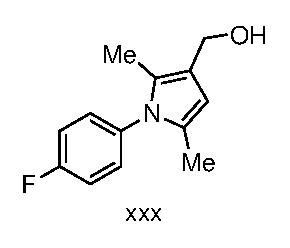
\includegraphics{exp/PMY15.eps}
	\end{center}
	\vspace{-25pt}	
	\end{figure}	

{\ce{LiAlH4} (72 mg, 1.91 mmol, 1 equiv, 4 hydride equiv.) was stirred in Et2O (5 mL) at room temperature (water bath). PMY 6-1 (500 mg, 1.91 mmol, 1 equiv.) in Et2O (10 mL) was added dropwise over 5 minutes. After 6 hours, a saturated solution of Rochelle's salt (approx 10 mL) was added, shaken and left to separate. Diluted with EtOAc (30 mL). Separated and aqueous extracted with EtOAc (3 × 20 mL), dried (MgSO4) and concentrated under reduced pressure. The residue was then purified by chromatography (2-30\% EtOAc/hexane) to obtain an off-white solid (264 mg, 63\%). 

Alternatively the product can be prepared from xxx carbaldehyde using \ce{NaBH4}.

%Mpt
Mpt.xxx--xxx $^\circ$C (xxx); 
%1H
$^1$H NMR (300 MHz, \ce{CDCl3}) $\delta$ 7.19--7.14 (m, 4H), 6.02 (s, 1H), 4.54 (s, 2H), 2.05 (s, 3H), 2.04 (s, 3H); 
%13C
  $^{13}$C NMR (75 MHz, \ce{CDCl3}) $\delta$ 162.0 (d, $J$ 247.4), 134.9 (d, $J$ 2.9), 130.0 (d, $J$ 8.6), 128.3, 126.7, 119.1, 116.1 (d, $J$ 22.7), 106.8, 57.7, 12.7, 10.5; 
%19F
$^{19}$F\{$^1$H\} NMR (282 MHz, \ce{CDCl3}) $\delta$ -113.62;
 %IR
 $\nu_{max}$ (neat) /$cm^{-1}$ ; 
%mass
\emph{m/z} (ESI+) xxx [M+H]$^+$.
%InChi
\seqsplit{InChi=1S/C13H14FNO/c1-9-7-11(8-16)10(2)15(9)13-5-3-12(14)4-6-13/h3-7,16H,8H2,1-2H3}. 
%experiment
See page \pageref{spec:PMY15} for NMR spectra.
\url{http://malaria.ourexperiment.org/uri/38}. \ce{NaBH4} \url{http://malaria.ourexperiment.org/uri/3e}

%\subsubsection*{OSM-S-12, PMY 20-1}

%Prepared according to General Procedure D


%Mpt
%Mpt.xxx--xxx $^\circ$C (xxx); 
%1H
%$^1$H NMR (300 MHz, \ce{CDCl3}) $\delta$ ; 
%13C
%  $^{13}$C NMR (75 MHz, \ce{CDCl3}) $\delta$ ; 
 %IR
% $\nu_{max}$ (neat) /$cm^{-1}$ ; 
%mass
%\emph{m/z} (ESI+) xxx [M+H]$^+$.
%InChi
%\seqsplit{InChi=1S/C13H13NO2/c1-9-8-12(13(15)16)10(2)14(9)11-6-4-3-5-7-11/h3-8H,1-2H3,(H,15,16)}. 
%experiment
%\url{http://malaria.ourexperiment.org/uri/42}. 


%\subsubsection*{OSM-S-13, PMY 21-1}

%Prepared according to General Procedure D


%Mpt
%Mpt.xxx--xxx $^\circ$C (xxx); 
%1H
%$^1$H NMR (300 MHz, \ce{CDCl3}) $\delta$ ; 
%13C
%  $^{13}$C NMR (75 MHz, \ce{CDCl3}) $\delta$ ; 
 %IR
% $\nu_{max}$ (neat) /$cm^{-1}$ ; 
%mass
%\emph{m/z} (ESI+) xxx [M+H]$^+$.
%InChi
%\seqsplit{InChi=1S/C14H15NO2/c1-9-4-6-12(7-5-9)15-10(2)8-13(11(15)3)14(16)17/h4-8H,1-3H3,(H,16,17)}. 
%experiment
%\url{http://malaria.ourexperiment.org/uri/43}. 

%\subsubsection*{OSM-S-14, PMY 22-1}

%Prepared according to General Procedure D


%Mpt
%Mpt.xxx--xxx $^\circ$C (xxx); 
%1H
%$^1$H NMR (300 MHz, \ce{CDCl3}) $\delta$ ; 
%13C
%$^{13}$C NMR (75 MHz, \ce{CDCl3}) $\delta$ ; 
 %IR
% $\nu_{max}$ (neat) /$cm^{-1}$ ; 
%mass
%\emph{m/z} (ESI+) xxx [M+H]$^+$.
%InChi
%\seqsplit{InChi=1S/C14H12F3NO2/c1-8-7-12(13(19)20)9(2)18(8)11-5-3-10(4-6-11)14(15,16)17/h3-7H,1-2H3,(H,19,20)}. 
%experiment
%\url{http://malaria.ourexperiment.org/uri/44}. 

\subsubsection*{OSM-S-19, PMY 31-5}
 \label{exp:PMY31}
	\begin{figure}[H]
	\begin{center}
	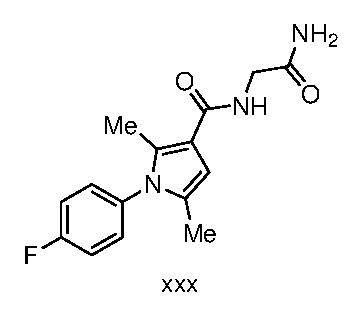
\includegraphics{exp/PMY31.eps}
	\end{center}
	\vspace{-25pt}	
	\end{figure}	

%Mpt
Mpt.193--195 $^\circ$C (xxx); 
%1H
$^1$H NMR (300 MHz, \ce{CDCl3}) $\delta$ ; 
%13C
  $^{13}$C NMR (75 MHz, \ce{CDCl3}) $\delta$ ; 
 %IR
 $\nu_{max}$ (neat) /$cm^{-1}$ ; 
%mass
\emph{m/z} (ESI+) 311 [M+Na]$^+$.
%InChi
\seqsplit{InChi=1S/C15H16FN3O2/c1-9-7-13(15(21)18-8-14(17)20)10(2)19(9)12-5-3-11(16)4-6-12/h3-7H,8H2,1-2H3,(H2,17,20)(H,18,21)}. 
%experiment
\url{http://malaria.ourexperiment.org/uri/8e}. 

\subsubsection*{OSM-S-20, PMY 32-3}
\label{exp:PMY32}
	\begin{figure}[H]
	\begin{center}
	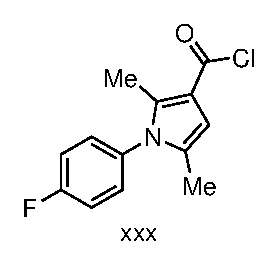
\includegraphics{exp/PMY32.eps}
	\end{center}
	\vspace{-25pt}	
	\end{figure}	

Prepared according to literature procedure.\url{http://www.wipo.int/patentscope/search/en/WO2006076202}
Used without further purification.

%1H
$^1$H NMR (300 MHz, \ce{CDCl3}) $\delta$ ; 
%13C
  $^{13}$C NMR (75 MHz, \ce{CDCl3}) $\delta$ ; 
 %IR
 $\nu_{max}$ (neat) /$cm^{-1}$ ; 
%mass
\emph{m/z} (ESI+) xxx [M+H]$^+$.
%InChi
\seqsplit{InChi=1S/C13H11ClFNO/c1-8-7-12(13(14)17)9(2)16(8)11-5-3-10(15)4-6-11/h3-7H,1-2H3}. 
%experiment
\url{http://malaria.ourexperiment.org/uri/bd}. 

\subsubsection*{OSM-S-21, PMY 34-1}
\label{exp:PMY34}
	\begin{figure}[H]
	\begin{center}
	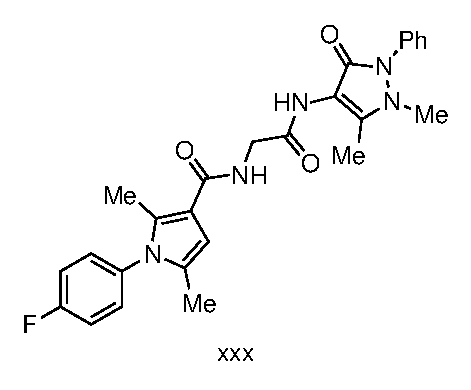
\includegraphics{exp/PMY34.eps}
	\end{center}
	\vspace{-25pt}	
	\end{figure}	

%Mpt
Mpt.xxx--xxx $^\circ$C (xxx); 
%1H
$^1$H NMR (300 MHz, \ce{CDCl3}) $\delta$ ; 
%13C
  $^{13}$C NMR (75 MHz, \ce{CDCl3}) $\delta$ ; 
 %IR
 $\nu_{max}$ (neat) /$cm^{-1}$ ; 
%mass
\emph{m/z} (ESI+) 498 [M+Na]$^+$.
%InChi
\seqsplit{InChi=1S/C26H26FN5O3/c1-16-14-22(17(2)31(16)20-12-10-19(27)11-13-20)25(34)28-15-23(33)29-24-18(3)30(4)32(26(24)35)21-8-6-5-7-9-21/h5-14H,15H2,1-4H3,(H,28,34)(H,29,33)}. 
%experiment
\url{http://malaria.ourexperiment.org/uri/8f}. 

%\subsubsection*{OSM-S-22, PMY 42-1}


%Mpt
%Mpt.xxx--xxx $^\circ$C (xxx); 
%1H
%$^1$H NMR (300 MHz, \ce{CDCl3}) $\delta$ ; 
%13C
 % $^{13}$C NMR (75 MHz, \ce{CDCl3}) $\delta$ ; 
 %IR
% $\nu_{max}$ (neat) /$cm^{-1}$ ; 
%mass
%\emph{m/z} (ESI+) xxx [M+H]$^+$.
%InChi
%\seqsplit{InChi=xxx}. 
%experiment
%\url{http://malaria.ourexperiment.org/xxx}. 

\subsubsection*{Synthesis of ethyl 2,5-dimethyl-1-($p$-tolyl)-1$H$-pyrrole-3-carboxylate, OSM-S-30, LMW 6-1}
\label{exp:LMW6}
	\begin{figure}[H]
	\begin{center}
	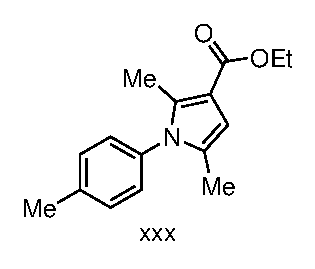
\includegraphics{exp/LMW6.eps}
	\end{center}
	\vspace{-25pt}	
	\end{figure}
 
=== standardise ===

Prepared according to general procedure C using ethyl acetoacetate (2 mL, 15.7 mmol, 1 equiv.) and \ce{K2CO3} (2.82 g, 20.4 mmol, 1.3 equiv.) in MeCN (30 mL) were mixed. Chloroacetone (1.6 mL, 17.2 mmol, 1.1 equiv.) and NaI (2.7 g, 18 mmol, 1.15 equiv.) were added and heated in an oil bath at 80 $^\circ$C. TLC showed reaction at completion after 2.5 hrs. After 3 hrs reflux, solution was allowed to cool to room temperature and then filtered and washed with EtOAc (30 mL). Mixture was concentrated under reduced pressure, dissolved in EtOAc (40 mL) and washed with water (20 mL), 1:1 water:brine (20 mL) and brine (20 mL). Crude product was then concentrated under reduced pressure. p-toluidine (2.02 g, 18.8 mmol, 1.2 equiv.) was added to crude intermediate and heated in an oil bath at 90 $^\circ$C. At 1.5 hrs, reaction was complete by TLC and reaction was allowed to cool to room temperature. Dark brown product was washed with EtOAc (2 $\times$ 20 mL), 10\% citric acid (3 $\times$ 20 mL), water (2 $\times$ 20 mL) and brine (20 mL) and then concentrated under reduced pressure to form a black oil. Product was dissolved in EtOH and activated charcoal added to remove coloured impurities. Product was stirred for 1 hr then filtered and washed with EtOH. Filtrate was concentrated under reduced pressure to form a black oil. Oil was purified by chromatography on silica (2-10\% EtOAc in petrol). Pure and impure fractions were taken separately and concentrated under reduced pressure to produce yellow and dark yellow oils respectively. Pure fraction crystallised overnight to a bright yellow crystalline solid (1.8 g, 45.6\%).
%Mpt
Mpt. 60--63 $^\circ$C (EtOAc/petrol); 
%1H
$^1$H NMR (300 MHz, \ce{CDCl3}) $\delta$  7.27 (d, $J$ 7.6, 2H), 7.04 (d, $J$ 7.6, 2H), 6.36 (s, 1H), 4.27 (q, $J$ 7.0, 2H), 2.42 (s, 3H), 2.28 (s, 3H), 1.96 (s, 3H), 1.34 (t, $J$ 7.0, 3H); 
%13C
  $^{13}$C NMR (75 MHz, \ce{CDCl3}) $\delta$ 165.8, 138.5, 136.3, 135.1, 130.0, 128.8, 127.9, 111.3, 107.4, 59.2, 21.2, 14.6, 12.6, 12.4; 
 %IR
 $\nu_{max}$ (neat) /$cm^{-1}$ 2982, 1693, 1515, 1411, 1218, 1081, 767; 
%mass
\emph{m/z} (APCI+) 258 [M+H]$^+$.
%InChi
\seqsplit{InChi=1S/C16H19NO2/c1-5-19-16(18)15-10-12(3)17(13(15)4)14-8-6-11(2)7-9-14/h6-10H,5H2,1-4H3}. 
%experiment
\url{http://malaria.ourexperiment.org/uri/4f}. 

\subsubsection*{ethyl 2,5-dimethyl-1-[$p$-(trifluoromethyl)phenyl]-1$H$-pyrrole-3-carboxylate, OSM-S-32, LMW 9}
\label{exp:LMW9}
	\begin{figure}[H]
	\begin{center}
	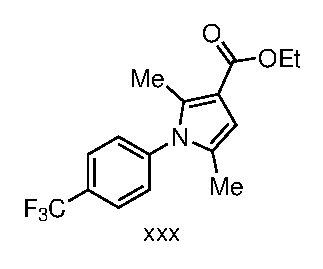
\includegraphics{exp/LMW9.eps}
	\end{center}
	\vspace{-25pt}	
	\end{figure}
	
=== standardise ===

Prepared according to general procedure xxx using ethyl acetoacetate (6 mL, 47 mmol, 1 equiv.) and \ce{K2CO3} (8.45 g, 61.1 mmol, 1.3 equiv.) were mixed in MeCN (55 mL). NaI (7.05 g, 47 mmol, 1 equiv.) and Chloroacetone (4.8 mL, 51.7 mmol, 1.1 equiv.) were added and mixture heated to 80oC in an oil bath. TLC at 2 hours showed reaction at completion. Reaction was allowed to cool to room temperature. Mixture washed with EtOAc (2 x 20 mL), water (2 x 20 mL), 1:1 water:brine (2 x 20 mL) and brine (2 x 20 mL) and dried with MgSO4 and concentrated under reduced pressure to form a yellow oil. Ethyl 2-acetyl-4-oxopentanoate intermediate (LMW 7-1) (2 mL, 10.7 mmol, 1 equiv.) was added to p-(trifluoromethyl)aniline (1.62 mL, 12.9 mmol, 1.2 equiv.) and heated at 80oC in an oil bath for 1.25 hrs. TLC at 1 hour showed reaction at completion and reaction was allowed to cool to room temperature. Product was washed with EtOAc (2 x 20 mL), 10\% citric acid (3 x 20 mL), water (20 mL) and brine (2 x 20 mL) and then concentrated under reduced pressure to form a dark brown oil. Brown oil was dissolved in 20 mL EtOH and heated before filtering under heat to remove residual salts and washing with hot EtOH. Filtrate was concentrated under reduced pressure and purified by chromatography on silica (2-15\% EtOAc in petrol). Pure fractions were taken and concentrated under reduced pressure to produce a light yellow oil. Product was cooled in a refrigerator overnight forming a pale yellow crystalline solid (1.85 g, 55\%).

%Mpt
Mpt. 66--68 $^\circ$C (EtOAc/petrol); 
%1H
$^1$H NMR (300 MHz, \ce{CDCl3}) $\delta$  7.78 (d, $J$  8.0, 2H), 7.33 (d, $J$ 8.0, 2H), 6.41 (s, 1H), 4.28 (q, $J$ 7.0, 2H), 2.30 (s, 3H), 1.99 (s, 3H), 1.35 (t, $J$ 7.0, 3H); 
%13C
  $^{13}$C NMR (75 MHz, \ce{CDCl3}) $\delta$ 165.5, 141.0, 135.9, 131.0 (q, $J$ 32.9), 128.8, 128.5, 126.6 (q, $J$ 3.3), 123.7 (q, $J$ 272.6), 112.2, 108.2, 59.4, 14.5, 12.7, 12.4; 
%19F
$^{19}$F NMR (282 MHz, \ce{CDCl3}): δ -62.7;
 %IR
 $\nu_{max}$ (neat) /$cm^{-1}$  2928, 1681, 1614, 1414, 1322, 1215, 120, 1065, 541, 770;
%mass
\emph{m/z} (APCI+) 312 [M+H]$^+$.
%InChi
\seqsplit{InChi=1S/C16H16F3NO2/c1-4-22-15(21)14-9-10(2)20(11(14)3)13-7-5-12(6-8-13)16(17,18)19/h5-9H,4H2,1-3H3}. 
%experiment
\url{http://malaria.ourexperiment.org/uri/51}. 

\subsubsection*{OSM-S-33, ZYH 1-1}
\label{exp:ZYH1}
	\begin{figure}[H]
	\begin{center}
	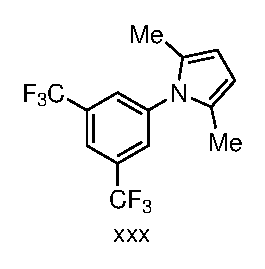
\includegraphics{exp/ZYH1.eps}
	\end{center}
	\vspace{-25pt}	
	\end{figure}


Prepared according to General Procedure A

%1H
$^1$H NMR (300 MHz, \ce{CDCl3}) $\delta$ 7.72 (d $J$ 0.3Hz, 2H, rotamers), 5.96 (br d, $J$ 1.7, 2H rotamers), 2.07 (br d, rotamers 6H); 
%13C
$^{13}$C NMR (75 MHz, \ce{CDCl3}) $\delta$ 140.9, 133.0 (q, $J$ 33.9), 128.8, 128.6 (q, $J$ 3.6), 123.1 (q $J$ 272.6), 121.5 (dq $J$ 3.5 and 3.8), 107.6, 13.1;
 %IR
 $\nu_{max}$ (neat) /$cm^{-1}$ 1713, 1621, 1410, 1274, 1124, 900, 682; 
%mass
\emph{m/z} HRES (APCI) high res mass, reported is for M-H2 + H. ?!?
%InChi
\seqsplit{InChi=1S/C14H11F6N/c1-8-3-4-9(2)21(8)12-6-10(13(15,16)17)5-11(7-12)14(18,19)20/h3-7H,1-2H3}. 
%experiment
\url{http://malaria.ourexperiment.org/uri/52}. 

\subsubsection*{OSM-S-34, ZYH 2-2}
\label{exp:ZYH2}
	\begin{figure}[H]
	\begin{center}
	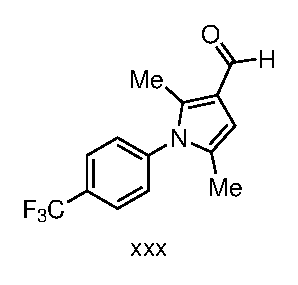
\includegraphics{exp/ZYH2.eps}
	\end{center}
	\vspace{-25pt}	
	\end{figure}


Prepared according to General Procedure B


%Mpt
Mpt. 85--87 $^\circ$C; 
%1H
$^1$H NMR (300 MHz, \ce{CDCl3}) $\delta$ 9.90 (s, 1H), 7.81 (d, $J$ 8.4, 2H), 7.36 (d, $J$ 8.4, 2H), 6.42 (s, 1H), 2.30 (s, 3H), 2.00 (s, 3H);
%13C
$^{13}$C NMR (75 MHz, \ce{CDCl3}) $\delta$  185.4, 140.3, 138.4, 131.3 (q, $J$ 32.9), 130.8, 128.7 (2C), 126.9 (q, $J$ 3.6), 123.7 (q, $J$ 272.4), 122.5 (2C), 106.6, 12.8, 11.3; 
 %IR
 $\nu_{max}$ (neat) /$cm^{-1}$ 16558, 1614, 1520, 1424, 1401, 1321; 
%mass
\emph{m/z} (ESI+ )268 [M+H]$^+$; HRES (ESI+) 290.07619  [M+Na]$^+$, \ce{C14H12F3NNaO} requires 290.07687.
%InChi
\seqsplit{InChi=1S/C14H12F3NO/c1-9-7-11(8-19)10(2)18(9)13-5-3-12(4-6-13)14(15,16)17/h3-8H,1-2H3}. 
%experiment
\url{http://malaria.ourexperiment.org/uri/58}. 

\subsubsection*{(2$Z$,5$Z$)-5-((2,5-dimethyl-1-phenyl-1$H$-pyrrol-3-yl)methylene)-2-(phenylimino)thiazolidin-4-one, OSM-S-35, ZYH 3-1}
\label{exp:ZYH3}
	\begin{figure}[H]
	\begin{center}
	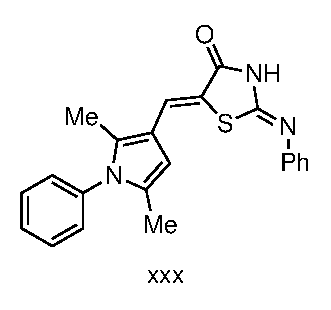
\includegraphics{exp/ZYH3.eps}
	\end{center}
	\vspace{-25pt}	
	\end{figure}
	
Prepared according to general procedure F


%Mpt
Mpt. 273 $^\circ$C (decomposes); 
%1H
$^1$H NMR (300 MHz, \ce{DMSO-d6}) $\delta$ ; 
%13C
  $^{13}$C NMR (75 MHz, \ce{CDCl3}) $\delta$ ; 
 %IR
 $\nu_{max}$ (neat) /$cm^{-1}$ 1703, 1637, 1591, 1495, 1300, 1173; 
%mass
\emph{m/z} (ESI+) 374 [M+H]$^+$; HRES (ESI+) 374.13105 [M+H]$^+$, \ce{C22H20N3OS} requires 374.13271.
%InChi
\seqsplit{InChi=1S/C22H19N3OS/c1-15-13-17(16(2)25(15)19-11-7-4-8-12-19)14-20-21(26)24-22(27-20)23-18-9-5-3-6-10-18/h3-14H,1-2H3,(H,23,24,26)/b20-14-}. 
%experiment
\url{http://malaria.ourexperiment.org/uri/54}. 

\subsubsection*{1-(3,5-bis(trifluoromethyl)phenyl)-2,5-dimethyl-1$H$-pyrrole-3-carbaldehyde, OSM-S-36, ZYH 4-2/4-3}
\label{exp:ZYH4}
	\begin{figure}[H]
	\begin{center}
	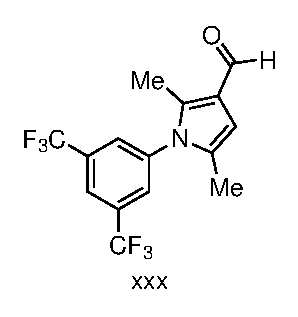
\includegraphics{exp/ZYH4.eps}
	\end{center}
	\vspace{-25pt}	
	\end{figure}
	
Prepared according to General Procedure B

%Mpt
Mpt. 95--96 $^\circ$C; 
%1H
$^1$H NMR (300 MHz, \ce{CDCl3}) $\delta$ 9.90 (s, 1H), 8.04 (s, 1H), 7.74 (s, 2H), 6.44 (app d, $J$ 0.7, rotamers, 1H), 2.33 (s, 3H), 2.03 (s, 3H);
%13C
  $^{13}$C NMR (75 MHz, \ce{CDCl3}) $\delta$ 185.4, 138.8, 138.0, 133.6 (q, $J$ 34.3, 2C), 130.6, 128.7 (q, $J$ 3.4, 2C), 123.0 (dq $J$ 3.8 and 3.9, 2C), 122.9, 122.7 (q, $J$ 273.1, 2C), 107.4, 12.8, 11.4;
 %IR
 $\nu_{max}$ (neat) /$cm^{-1}$ ; 
%mass
\emph{m/z} HRES (ESI+) found 336.08190 [M+H]$^+$, \ce{C15H11F6NO} requires 336.08176.
%InChi
\seqsplit{InChi=1S/C15H11F6NO/c1-8-3-10(7-23)9(2)22(8)13-5-11(14(16,17)18)4-12(6-13)15(19,20)21/h3-7H,1-2H3}. 
%experiment
\url{http://malaria.ourexperiment.org/uri/55}. 

\subsubsection*{(2$Z$,5$Z$4)-5-((2,5-dimethyl-1-(p-tolyl)-1$H$-pyrrol-3-yl)methylene)-2-(phenylimino)thiazolidin-4-one, OSM-S-37, ZYH 5-1}
\label{exp:ZYH5}
	\begin{figure}[H]
	\begin{center}
	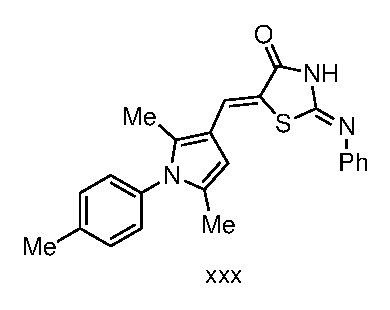
\includegraphics{exp/ZYH5.eps}
	\end{center}
	\vspace{-25pt}	
	\end{figure}

Prepared according to general procedure F

%Mpt
Mpt. 279 $^\circ$C (decomposes); 
%1H
$^1$H NMR (300 MHz, \ce{CDCl3}) $\delta$ ; 
%13C
  $^{13}$C NMR (75 MHz, \ce{CDCl3}) $\delta$ ; 
 %IR
 $\nu_{max}$ (neat) /$cm^{-1}$ ; 
%mass
\emph{m/z} (ESI+) 388 [M+H]$^+$; HRES (ESI+) found 388.14765 [M+H]$^+$, \ce{C23H22N3OS} requires 388.14836.
%InChi
\seqsplit{InChi=1S/C23H21N3OS/c1-15-9-11-20(12-10-15)26-16(2)13-18(17(26)3)14-21-22(27)25-23(28-21)24-19-7-5-4-6-8-19/h4-14H,1-3H3,(H,24,25,27)/b21-14-}. 
%experiment
\url{http://malaria.ourexperiment.org/uri/56}. 

\subsubsection*{\seqsplit{(2$Z$,5$Z$)-5-((2,5-dimethyl-1-(4-(trifluoromethyl)phenyl)-1$H$-pyrrol-3-yl)methylene)-2-(phenylimino)thiazolidin-4-one, OSM-S-38, ZYH 6}}
\label{exp:ZYH6}
	\begin{figure}[H]
	\begin{center}
	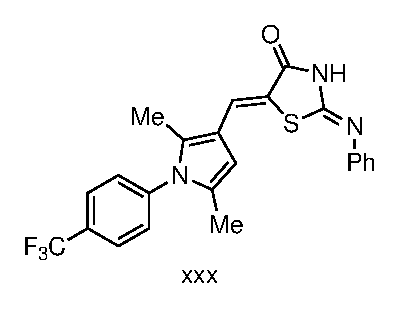
\includegraphics{exp/ZYH6.eps}
	\end{center}
	\vspace{-25pt}	
	\end{figure}

Prepared according to general procedure F

%Mpt
Mpt. 308 $^\circ$C (decomp); 
%1H
$^1$H NMR (300 MHz, \ce{CDCl3}) $\delta$ ; 
%13C
 $^{13}$C NMR (75 MHz, \ce{CDCl3}) $\delta$ ; 
%IR
 $\nu_{max}$ (neat) /$cm^{-1}$ ; 
%mass
\emph{m/z} (ESI+) xxx [M+H]$^+$.
%InChi
\seqsplit{InChi=1S/C23H18F3N3OS/c1-14-12-16(15(2)29(14)19-10-8-17(9-11-19)23(24,25)26)13-20-21(30)28-22(31-20)27-18-6-4-3-5-7-18/h3-13H,1-2H3,(H,27,28,30)/b20-13-}. 
%experiment
\url{http://malaria.ourexperiment.org/uri/59}. 

\subsubsection*{OSM-S-39, ZYH 7-2}
\label{exp:ZYH7}
	\begin{figure}[H]
	\begin{center}
	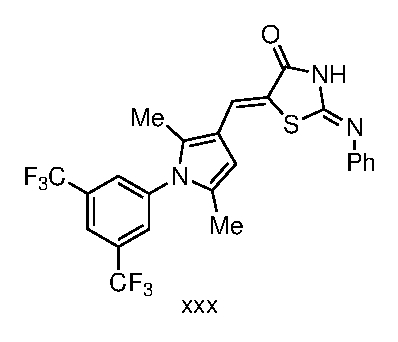
\includegraphics{exp/ZYH7.eps}
	\end{center}
	\vspace{-25pt}	
	\end{figure}

Prepared according to general procedure F


%Mpt
Mpt. 255 (decomposes) $^\circ$C; 
%1H
$^1$H NMR (300 MHz, \ce{CDCl3}) $\delta$ ; 
%13C
  $^{13}$C NMR (75 MHz, \ce{CDCl3}) $\delta$ ; 
 %IR
 $\nu_{max}$ (neat) /$cm^{-1}$ ; 
%mass
\emph{m/z} HRES (ESI+) 510.10796 [M+H]$^+$, \ce{C24H18F6N3OS} requires 510.10748.
%InChi
\seqsplit{InChi=1S/C24H17F6N3OS/c1-13-8-15(9-20-21(34)32-22(35-20)31-18-6-4-3-5-7-18)14(2)33(13)19-11-16(23(25,26)27)10-17(12-19)24(28,29)30/h3-12H,1-2H3,(H,31,32,34)/b20-9-.} 
%experiment
\url{http://malaria.ourexperiment.org/uri/64}. 

\subsubsection*{OSM-S-40, ZYH 8-1}
\label{exp:ZYH8}
	\begin{figure}[H]
	\begin{center}
	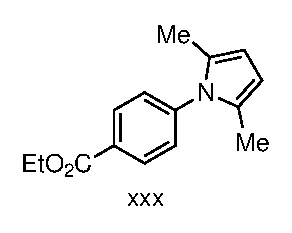
\includegraphics{exp/ZYH8.eps}
	\end{center}
	\vspace{-25pt}	
	\end{figure}

Prepared according to General Procedure A


%Mpt
Mpt. 60--61 $^\circ$C; 
%1H
$^1$H NMR (300 MHz, \ce{CDCl3}) $\delta$ ; 
%13C
  $^{13}$C NMR (75 MHz, \ce{CDCl3}) $\delta$ ; 
 %IR
 $\nu_{max}$ (neat) /$cm^{-1}$ ; 
%mass
\emph{m/z} (APCI) 244 [M+H]$^+$.
%InChi
\seqsplit{InChi=1S/C15H17NO2/c1-4-18-15(17)13-7-9-14(10-8-13)16-11(2)5-6-12(16)3/h5-10H,4H2,1-3H3}. 
%experiment
\url{http://malaria.ourexperiment.org/uri/5f}. 

\subsubsection*{OSM-S-42, ZYH 10-1 A}
\label{exp:ZYH10A}
	\begin{figure}[H]
	\begin{center}
	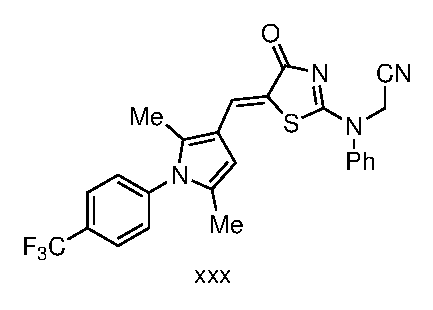
\includegraphics{exp/ZYH10A.eps}
	\end{center}
	\vspace{-25pt}	
	\end{figure}

%Mpt
Mpt. 182--183 $^\circ$C; 
%1H
$^1$H NMR (300 MHz, \ce{CDCl3}) $\delta$ ; 
%13C
  $^{13}$C NMR (75 MHz, \ce{CDCl3}) $\delta$ ; 
 %IR
 $\nu_{max}$ (neat) /$cm^{-1}$ ; 
%mass
\emph{m/z} (ESI+) 982 [2M+Na]$^+$;  HRES (ESI+) 503.11264 [M+Na]$^+$, \ce{C25H19F3N4NaOS} requires 503.11294.
%InChi
\seqsplit{InChi=1S/C25H19F3N4OS/c1-16-14-18(17(2)32(16)21-10-8-19(9-11-21)25(26,27)28)15-22-23(33)30-24(34-22)31(13-12-29)20-6-4-3-5-7-20/h3-11,14-15H,13H2,1-2H3/b22-15-}. 
%experiment
\url{http://malaria.ourexperiment.org/uri/61}. 

\subsubsection*{OSM-S-43, ZYH 10-1 B}
\label{exp:ZYH10B}
	\begin{figure}[H]
	\begin{center}
	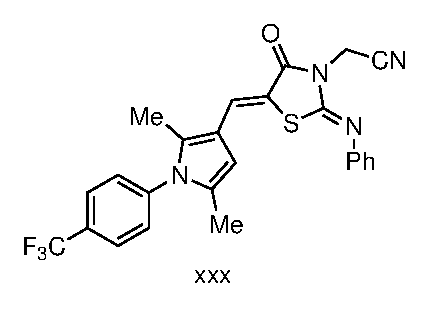
\includegraphics{exp/ZYH10B.eps}
	\end{center}
	\vspace{-25pt}	
	\end{figure}

%Mpt
Mpt. 72--74 $^\circ$C (xxx); 
%1H
$^1$H NMR (300 MHz, \ce{CDCl3}) $\delta$ ; 
%13C
  $^{13}$C NMR (75 MHz, \ce{CDCl3}) $\delta$ ; 
 %IR
 $\nu_{max}$ (neat) /$cm^{-1}$ ; 
%mass
\emph{m/z} (ESI+) 503 [M+Na]$^+$; HRES (ESI+) 503.11295 [M+Na]$^+$, \ce{C25H19F3N4NaOS} requires 503.11294.
%InChi
\seqsplit{InChi=1S/C25H19F3N4OS/c1-16-14-18(17(2)32(16)21-10-8-19(9-11-21)25(26,27)28)15-22-23(33)31(13-12-29)24(34-22)30-20-6-4-3-5-7-20/h3-11,14-15H,13H2,1-2H3/b22-15-,30-24-}. 
%experiment
\url{http://malaria.ourexperiment.org/uri/61}. 

\subsubsection*{OSM-S-44, ZYH 11-1}
\label{exp:ZYH11}
	\begin{figure}[H]
	\begin{center}
	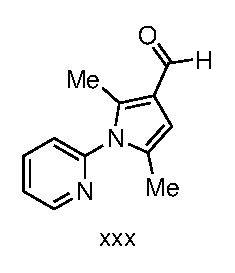
\includegraphics{exp/ZYH11.eps}
	\end{center}
	\vspace{-25pt}	
	\end{figure}

Prepared accoding to General Procedure B

%Mpt
Mpt. 61--64 $^\circ$C; 
%1H
$^1$H NMR (300 MHz, \ce{CDCl3}) $\delta$ ; 
%13C
  $^{13}$C NMR (75 MHz, \ce{CDCl3}) $\delta$ ; 
 %IR
 $\nu_{max}$ (neat) /$cm^{-1}$ ; 
%mass
\emph{m/z} HRES (APCI) 201.10165 [M+H]$^+$, \ce{C12H13N2O} requires 201.10279.
%InChi
\seqsplit{InChi=1S/C12H12N2O/c1-9-7-11(8-15)10(2)14(9)12-5-3-4-6-13-12/h3-8H,1-2H3}. 
%experiment
\url{http://malaria.ourexperiment.org/uri/67}. 

\subsubsection*{ZYH 12-1/12-2}
\label{exp:ZYH12}
	\begin{figure}[H]
	\begin{center}
	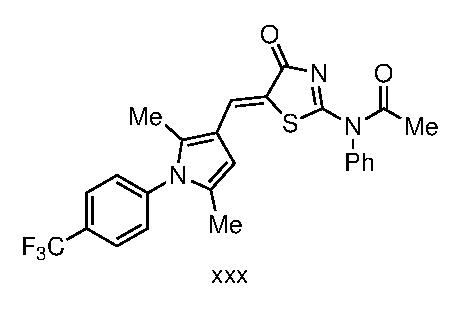
\includegraphics{exp/ZYH12.eps}
	\end{center}
	\vspace{-25pt}	
	\end{figure}

%Mpt
Mpt. 309--311 $^\circ$C; 
%1H
$^1$H NMR (300 MHz, \ce{CDCl3}) $\delta$ ; 
%13C
  $^{13}$C NMR (75 MHz, \ce{CDCl3}) $\delta$ ; 
 %IR
 $\nu_{max}$ (neat) /$cm^{-1}$ ; 
%mass
\emph{m/z} HRES (ESI+) 506.11167 [M+Na]$^+$, \ce{C25H20F3N3NaO2S} requires 506.11260.
%InChi
\seqsplit{InChi=1S/C25H20F3N3O2S/c1-15-13-18(16(2)30(15)21-11-9-19(10-12-21)25(26,27)28)14-22-23(33)31(17(3)32)24(34-22)29-20-7-5-4-6-8-20/h4-14H,1-3H3/b22-14+,29-24-}. 
%experiment
\url{http://malaria.ourexperiment.org/uri/74}.

\subsubsection*{OSM-S-46, ZYH 13-1}
\label{exp:ZYH13}
	\begin{figure}[H]
	\begin{center}
	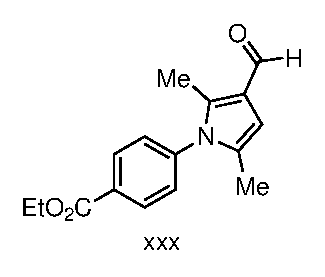
\includegraphics{exp/ZYH13.eps}
	\end{center}
	\vspace{-25pt}	
	\end{figure}

%Mpt
Mpt. 112--114 $^\circ$C; 
%1H
$^1$H NMR (300 MHz, \ce{CDCl3}) $\delta$ ; 
%13C
  $^{13}$C NMR (75 MHz, \ce{CDCl3}) $\delta$ ; 
 %IR
 $\nu_{max}$ (neat) /$cm^{-1}$ ; 
%mass
\emph{m/z} (APCI) 272 [M+H]$^+$.
%InChi
\seqsplit{InChi=1S/C16H17NO3/c1-4-20-16(19)13-5-7-15(8-6-13)17-11(2)9-14(10-18)12(17)3/h5-10H,4H2,1-3H3}. 
%experiment
\url{http://malaria.ourexperiment.org/uri/69}. 

\subsubsection*{OSM-S-47, ZYH 14-1}
\label{exp:ZYH14}
	\begin{figure}[H]
	\begin{center}
	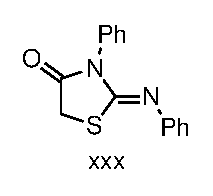
\includegraphics{exp/ZYH14.eps}
	\end{center}
	\vspace{-25pt}	
	\end{figure}

%Mpt
Mpt. 175--176 $^\circ$C; 
%1H
$^1$H NMR (300 MHz, \ce{CDCl3}) $\delta$ ; 
%13C
  $^{13}$C NMR (75 MHz, \ce{CDCl3}) $\delta$ ; 
 %IR
 $\nu_{max}$ (neat) /$cm^{-1}$ ; 
%mass
\emph{m/z} (APCI) 269 [M+H]$^+$.
%InChi
\seqsplit{InChi=1S/C15H12N2OS/c18-14-11-19-15(16-12-7-3-1-4-8-12)17(14)13-9-5-2-6-10-13/h1-10H,11H2/b16-15-}. 
%experiment
\url{http://malaria.ourexperiment.org/uri/70}. 

\subsubsection*{OSM-S-48, ZYH 15-1}
\label{exp:ZYH15}
	\begin{figure}[H]
	\begin{center}
	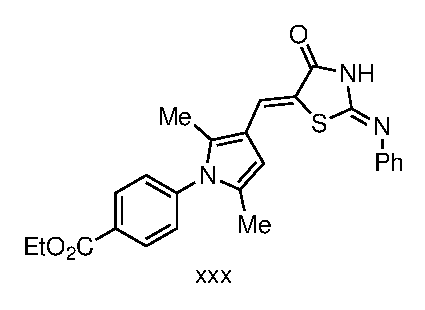
\includegraphics{exp/ZYH15.eps}
	\end{center}
	\vspace{-25pt}	
	\end{figure}

Prepared according to general procedure F

%Mpt
Mpt. 248 $^\circ$C (decomposes); 
%1H
$^1$H NMR (300 MHz, \ce{CDCl3}) $\delta$ ; 
%13C
  $^{13}$C NMR (75 MHz, \ce{CDCl3}) $\delta$ ; 
 %IR
 $\nu_{max}$ (neat) /$cm^{-1}$ ; 
%mass
\emph{m/z} (ESI+) 913 [2M+Na]$^+$; HRES (ESI+) 468.13527 [M+Na]$^+$, \ce{C25H23N3NaO3S} requires 468.13578.
%InChi
\seqsplit{InChi=1S/C25H23N3O3S/c1-4-31-24(30)18-10-12-21(13-11-18)28-16(2)14-19(17(28)3)15-22-23(29)27-25(32-22)26-20-8-6-5-7-9-20/h5-15H,4H2,1-3H3,(H,26,27,29)/b22-15-}. 
%experiment
\url{http://malaria.ourexperiment.org/uri/71}. 

\subsubsection*{OSM-S-49, ZYH 16-1}
\label{exp:ZYH16}
	\begin{figure}[H]
	\begin{center}
	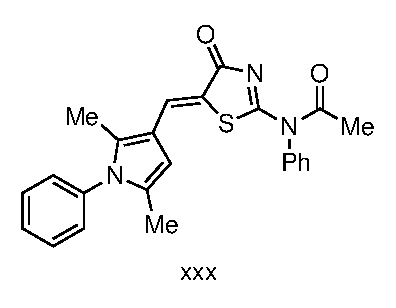
\includegraphics{exp/ZYH16.eps}
	\end{center}
	\vspace{-25pt}	
	\end{figure}

%Mpt
Mpt. 237--238 $^\circ$C; 
%1H
$^1$H NMR (300 MHz, \ce{CDCl3}) $\delta$ ; 
%13C
  $^{13}$C NMR (75 MHz, \ce{CDCl3}) $\delta$ ; 
 %IR
 $\nu_{max}$ (neat) /$cm^{-1}$ ; 
%mass
\emph{m/z} HRES (ESI+) 416.14285 [M+H]$^+$, \ce{C24H22N3O2S} requires 416.14327.
%InChi
\seqsplit{InChi=1S/C24H21N3O2S/c1-16-14-19(17(2)26(16)21-12-8-5-9-13-21)15-22-23(29)27(18(3)28)24(30-22)25-20-10-6-4-7-11-20/h4-15H,1-3H3/b22-15-,25-24-}. 
%experiment
\url{http://malaria.ourexperiment.org/uri/77}. 

\subsubsection*{OSM-S-50, ZYH 17-1}
\label{exp:ZYH17}
	\begin{figure}[H]
	\begin{center}
	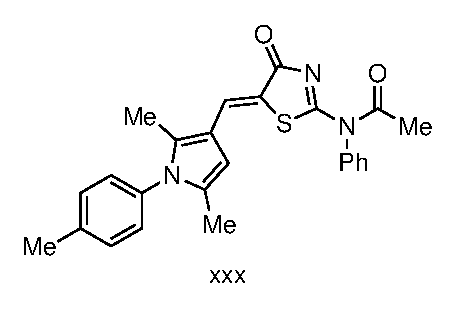
\includegraphics{exp/ZYH17.eps}
	\end{center}
	\vspace{-25pt}	
	\end{figure}

%Mpt
Mpt. 256--258 $^\circ$C; 
%1H
$^1$H NMR (300 MHz, \ce{CDCl3}) $\delta$ ; 
%13C
  $^{13}$C NMR (75 MHz, \ce{CDCl3}) $\delta$ ; 
 %IR
 $\nu_{max}$ (neat) /$cm^{-1}$ ; 
%mass
\emph{m/z} HRES (ESI+) 388.14793 [M-\ce{C2H3O}+H]$^+$, \ce{C23H22N3OS} requires 388.14836.
%InChi
\seqsplit{InChi=1S/C25H23N3O2S/c1-16-10-12-22(13-11-16)27-17(2)14-20(18(27)3)15-23-24(30)28(19(4)29)25(31-23)26-21-8-6-5-7-9-21/h5-15H,1-4H3/b23-15-,26-25-}. 
%experiment
\url{http://malaria.ourexperiment.org/uri/78}. 

\subsubsection*{OSM-S-51, ZYH 18-1}
\label{exp:ZYH18}
\begin{figure}[H]
	\begin{center}
	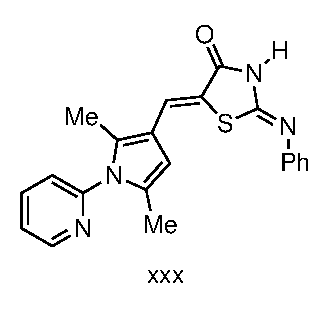
\includegraphics{exp/ZYH18.eps}
	\end{center}
	\vspace{-25pt}	
	\end{figure}


Prepared according to general procedure F

%Mpt
Mpt. 276--278 $^\circ$C; 
%1H
$^1$H NMR (300 MHz, \ce{CDCl3}) $\delta$ ; 
%13C
  $^{13}$C NMR (75 MHz, \ce{CDCl3}) $\delta$ ; 
 %IR
 $\nu_{max}$ (neat) /$cm^{-1}$ ; 
%mass
\emph{m/z} (ESI+) 397 [M+Na]$^+$; HRES (ESI+) 375.12680 [M+H]$^+$, \ce{C21H19N4OS} requires 375.12796.
%InChi
\seqsplit{InChi=1S/C21H18N4OS/c1-14-12-16(15(2)25(14)19-10-6-7-11-22-19)13-18-20(26)24-21(27-18)23-17-8-4-3-5-9-17/h3-13H,1-2H3,(H,23,24,26)/b18-13-}. 
%experiment
\url{http://malaria.ourexperiment.org/uri/79}. 

\subsubsection*{OSM-S-52, ZYH 19-1}
\label{exp:ZYH19}
\begin{figure}[H]
	\begin{center}
	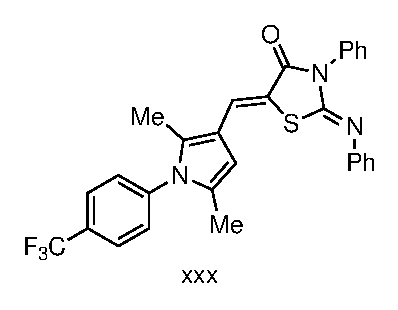
\includegraphics{exp/ZYH19.eps}
	\end{center}
	\vspace{-25pt}	
	\end{figure}

Prepared according to general procedure F

%Mpt
Mpt. 226--227 $^\circ$C; 
%1H
$^1$H NMR (300 MHz, \ce{CDCl3}) $\delta$ ; 
%13C
  $^{13}$C NMR (75 MHz, \ce{CDCl3}) $\delta$ ; 
 %IR
 $\nu_{max}$ (neat) /$cm^{-1}$ ; 
%mass
\emph{m/z} (ESI+) 540 [M+Na]$^+$; HRES (ESI+) 540.13240 [M+Na]$^+$, \ce{C29H22F3N3NaOS} requires 540.13334.
%InChi
\seqsplit{InChi=1S/C29H22F3N3OS/c1-19-17-21(20(2)34(19)25-15-13-22(14-16-25)29(30,31)32)18-26-27(36)35(24-11-7-4-8-12-24)28(37-26)33-23-9-5-3-6-10-23/h3-18H,1-2H3/b26-18-,33-28-}. 
%experiment
\url{http://malaria.ourexperiment.org/uri/7a}. 

\subsubsection*{OSM-S-54, ZYH 22-3}
\label{exp:ZYH22}
\begin{figure}[H]
	\begin{center}
	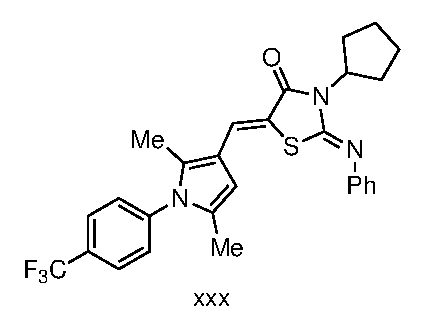
\includegraphics{exp/ZYH22.eps}
	\end{center}
	\vspace{-25pt}	
	\end{figure}

%Mpt
Mpt. 71--72 $^\circ$C; 
%1H
$^1$H NMR (300 MHz, \ce{CDCl3}) $\delta$ ; 
%13C
  $^{13}$C NMR (75 MHz, \ce{CDCl3}) $\delta$ ; 
 %IR
 $\nu_{max}$ (neat) /$cm^{-1}$ ; 
%mass
\emph{m/z} HRES (ESI+) 510.18203 [M+H]$^+$, \ce{C28H27F3N3OS} requires 510.18269.
%InChi
\seqsplit{InChi=1S/C28H26F3N3OS/c1-18-16-20(19(2)33(18)24-14-12-21(13-15-24)28(29,30)31)17-25-26(35)34(23-10-6-7-11-23)27(36-25)32-22-8-4-3-5-9-22/h3-5,8-9,12-17,23H,6-7,10-11H2,1-2H3/b25-17-,32-27-}. 
%experiment
\url{http://malaria.ourexperiment.org/uri/83}. 

\section{NMR Spectra}

\newpage

\subsubsection*{PMY 1, 1-(4-fluorophenyl)-2,5-dimethyl-1\emph{H}-pyrrole,l page \pageref{exp:PMY1}}
\label{spec:PMY1}
	\begin{figure}[H] 
	\begin{center}
	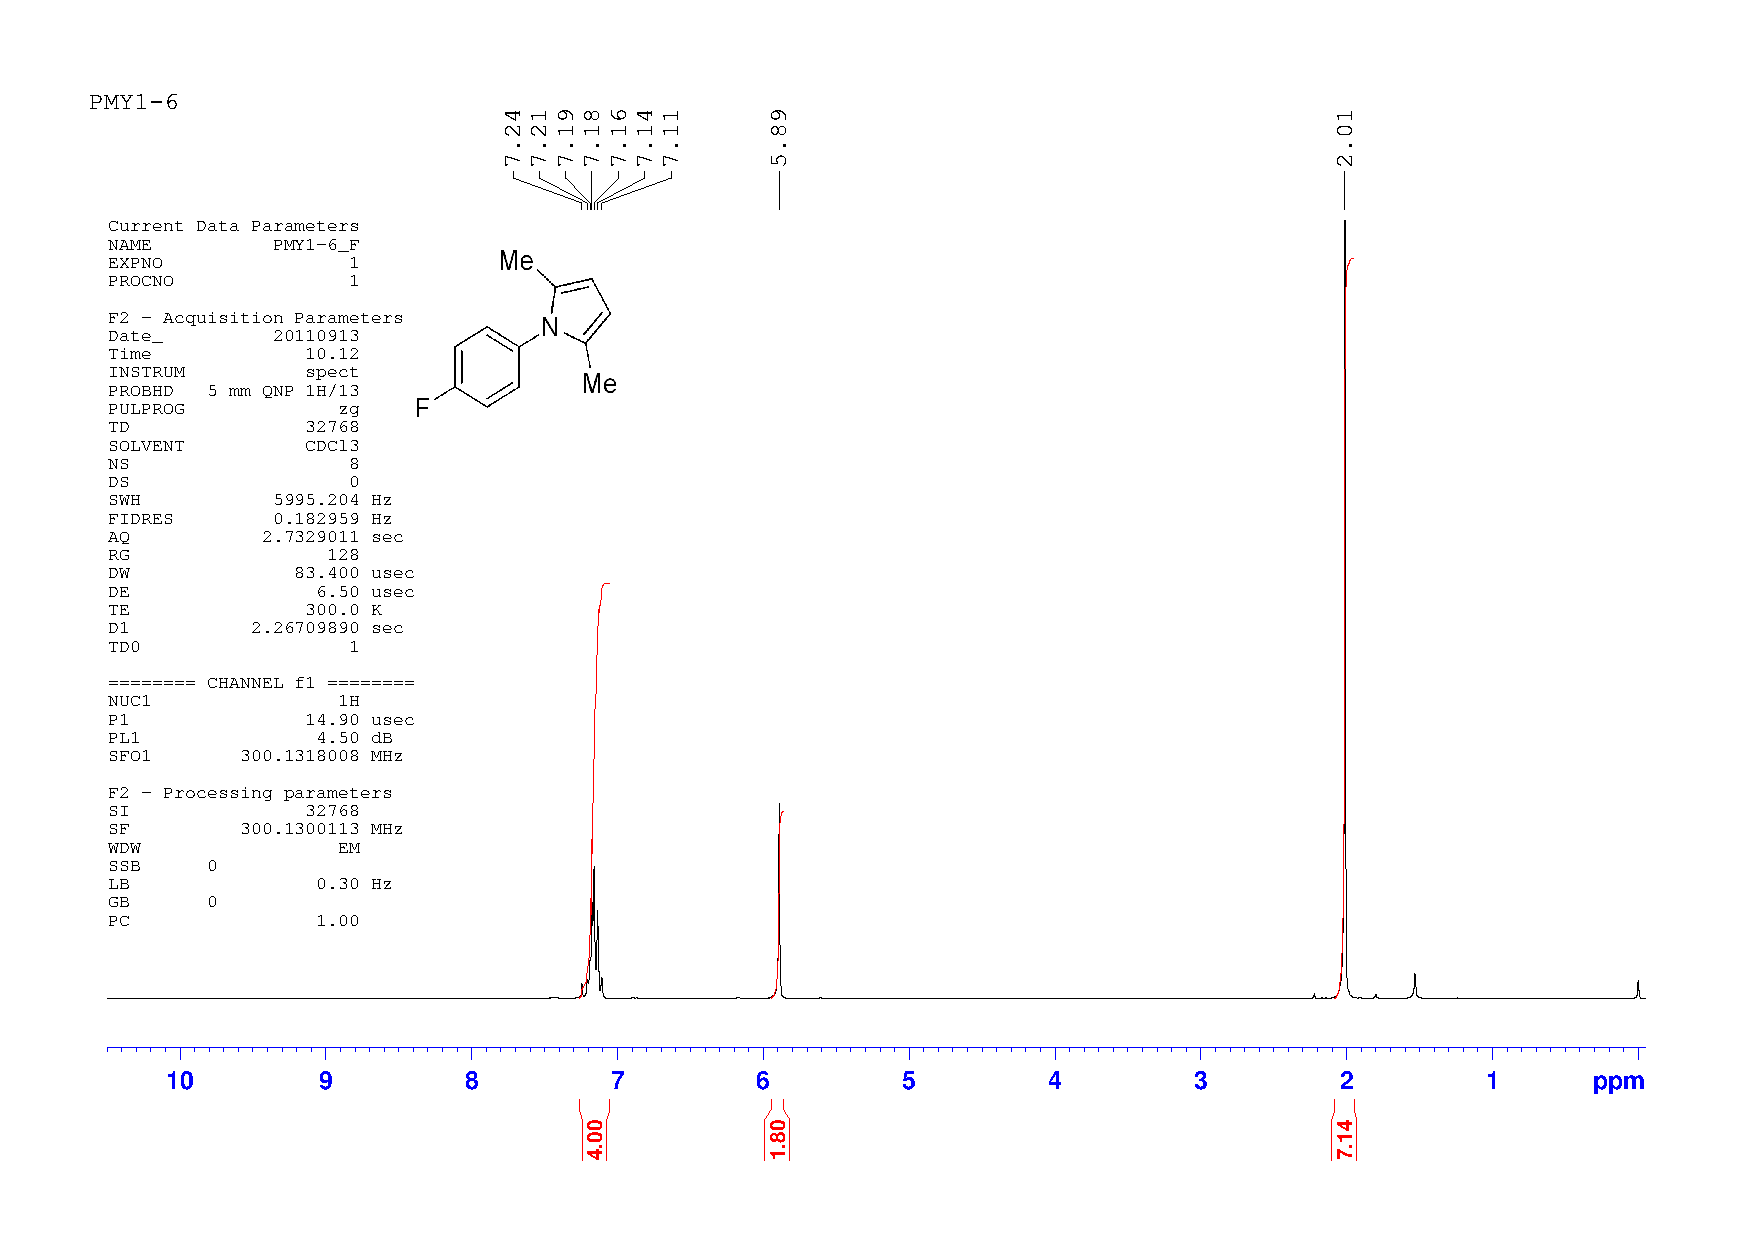
\includegraphics[width=14.5cm]{expdata/PMY1/1H}
	\includegraphics[width=14.5cm]{expdata/PMY1/13C}
	\end{center}
	\end{figure}

\subsubsection*{PMY 2, 1-(4-fluorophenyl)-2,5-dimethyl-1\emph{H}-pyrrole-3-carbaldehyde, page \pageref{exp:PMY2}}
\label{spec:PMY2}
	\begin{figure}[H] 
	\begin{center}
	\includegraphics[width=14.5cm]{expdata/PMY2/1H}
	\includegraphics[width=14.5cm]{expdata/PMY2/13C}
	\end{center}
	\end{figure}

\subsubsection*{PMY 26-1}

\subsubsection*{PMY 27-2}

\subsubsection*{PMY 29-1, PMY 29-2}

\subsubsection*{PMY 30-3}

%\subsubsection*{PMY 43-1}

%\subsubsection*{PMY 44-1}

\subsubsection*{LMW 1, \pageref{exp:LMW1}}
\label{spec:LMW1}
	\begin{figure}[H] 
	\begin{center}
	\includegraphics[width=14.5cm]{expdata/LMW1/1H}
	\includegraphics[width=14.5cm]{expdata/LMW1/13C}
	\end{center}
	\end{figure}

\subsubsection*{LMW 2, \pageref{exp:LMW2}}
\label{spec:LMW2}
	\begin{figure}[H] 
	\begin{center}
	\includegraphics[width=14.5cm]{expdata/LMW2/1H}
	\includegraphics[width=14.5cm]{expdata/LMW2/13C}
	\end{center}
	\end{figure}


\subsubsection*{LMW 3, \pageref{exp:LMW3}}
\label{spec:LMW3}
	\begin{figure}[H] 
	\begin{center}
	\includegraphics[width=14.5cm]{expdata/LMW3/1H}
	\includegraphics[width=14.5cm]{expdata/LMW3/13C}
	\end{center}
	\end{figure}

\subsubsection*{LMW 4-1, \pageref{exp:LMW4}}
\label{spec:LMW4}
	\begin{figure}[H] 
	\begin{center}
	\includegraphics[width=14.5cm]{expdata/LMW4/1H}
	\includegraphics[width=14.5cm]{expdata/LMW4/13C}
	\end{center}
	\end{figure}

\subsubsection*{LMW 5-1, \pageref{exp:LMW5}}
\label{spec:LMW5}
	\begin{figure}[H] 
	\begin{center}
	\includegraphics[width=14.5cm]{expdata/LMW5/1H}
	\includegraphics[width=14.5cm]{expdata/LMW5/13C}
	\end{center}
	\end{figure}

\subsubsection*{LMW 8-1}

\subsubsection*{ZYH 9-1}

\subsubsection*{ZYH 20-1}

\subsubsection*{ZYH 23-1}

\subsubsection*{OSM-S-3, PMY 6-1, ethyl 1-(4-fluorophenyl)-2,5-dimethyl-1$H$-pyrrole-3-carboxylate, page \pageref{exp:PMY6}}
\label{spec:PMY6}
	\begin{figure}[H] 
	\begin{center}
	\includegraphics[width=14.5cm]{expdata/PMY6/1H}
	\includegraphics[width=14.5cm]{expdata/PMY6/13C}
	\end{center}
	\end{figure}

\subsubsection*{OSM-S-8, PMY 8-2, 1-(4-fluorophenyl)-2,5-dimethyl-1$H$-pyrrole-3-carboxylic acid, page \pageref{exp:PMY8}}
\label{spec:PMY8}
	\begin{figure}[H] 
	\begin{center}
	\includegraphics[width=14.5cm]{expdata/PMY8/1H}
	\includegraphics[width=14.5cm]{expdata/PMY8/13C}
	\end{center}
	\end{figure}

\subsubsection*{OSM-S-5, PMY 10, TCMDC-123812, page \pageref{exp:PMY10}}
\label{spec:PMY10}
	\begin{figure}[H] 
	\begin{center}
	\includegraphics[width=14.5cm]{expdata/PMY10/1H}
	\includegraphics[width=14.5cm]{expdata/PMY10/13C}
	\end{center}
	\end{figure}

\subsubsection*{PMY 11-2}

\subsubsection*{PMY 12-1, page \pageref{exp:PMY12-1}}
\label{spec:PMY12-1}
	\begin{figure}[H] 
	\begin{center}
	\includegraphics[width=14.5cm]{expdata/PMY12-1/1H}
	\includegraphics[width=14.5cm]{expdata/PMY12-1/13C}
	\end{center}
	\end{figure}

\subsubsection*{PMY 12-5}

\subsubsection*{OSM-S-10, PMY 14-4}

\subsubsection*{OSM-S-9, PMY 35}
\label{spec:PMY35}
	\begin{figure}[H] 
	\begin{center}
	\includegraphics[width=14.5cm]{expdata/PMY35/1H}
	\includegraphics[width=14.5cm]{expdata/PMY35/13C}
	\end{center}
	\end{figure}

\subsubsection*{PMY 18-3, PMY 15-2, page \pageref{exp:PMY15}}
\label{spec:PMY15}
	\begin{figure}[H] 
	\begin{center}
	\includegraphics[width=14.5cm]{expdata/PMY15/1H}
	\includegraphics[width=14.5cm]{expdata/PMY15/13C}
	\end{center}
	\end{figure}

%\subsubsection*{PMY 20-1}

%\subsubsection*{PMY 21-1}

%\subsubsection*{PMY 22-1}

\subsubsection*{PMY 31-5}

\subsubsection*{PMY 32-3}

\subsubsection*{PMY 34-1}

%\subsubsection*{PMY 42-1}

\subsubsection*{LMW 6-1}

\subsubsection*{LMW 9-1}

\subsubsection*{ZYH 1-1}

\subsubsection*{ZYH 2-2}

\subsubsection*{ZYH 3-1, PMY 47-1}

\subsubsection*{ZYH 4-2/4-3}

\subsubsection*{ZYH 5-1}

\subsubsection*{ZYH 6-1/6-2}

\subsubsection*{ZYH 7-2}

\subsubsection*{ZYH 8-1}

\subsubsection*{ZYH 10-1 A}

\subsubsection*{ZYH 10-1 B}

\subsubsection*{ZYH 11-1}

\subsubsection*{ZYH 12-1/12-2}

\subsubsection*{ZYH 13-1}

\subsubsection*{ZYH 14-1}

\subsubsection*{ZYH 15-1}

\subsubsection*{ZYH 16-1}

\subsubsection*{ZYH 17-1}

\subsubsection*{ZYH 18-1}

\subsubsection*{ZYH 19-1}

\subsubsection*{ZYH 22-3}

\section{Single Crystal X-ray Data}

		\renewcommand{\bibname}{References}
		\bibliographystyle{bibstyle}
		\bibliography{refs}
	

	\end{document}